% =============================================================================
%  Memory in Levy walks from the dynamic-entropy formalism
%  A. Barra, A. Ladiana -- manuscript for Physical Review E (REVTeX 4.2)
%
%  Build:   pdflatex main && bibtex main && pdflatex main && pdflatex main
%  Figures: scripts/make_figs.py (from ../results/*.json and data/*.json)
% =============================================================================

\documentclass[aps,pre,twocolumn,superscriptaddress,floatfix,longbibliography,nofootinbib]{revtex4-2}
\usepackage[T1]{fontenc}
\usepackage[utf8]{inputenc}
\usepackage{newtxtext}
\usepackage{newtxmath}
\usepackage{amsmath}
\usepackage{bm}
\usepackage{graphicx}
\usepackage{dcolumn}
\usepackage{booktabs}
\usepackage{array}
\usepackage{xcolor}
\usepackage{microtype}
\definecolor{linkblue}{HTML}{2A3E78}
\usepackage[colorlinks=true,linkcolor=linkblue,citecolor=linkblue,urlcolor=linkblue]{hyperref}

\newcommand{\lmin}{\ell_{\min}}
\newcommand{\lmax}{\ell_{\max}}
\newcommand{\Lang}{\mathcal{L}}
\newcommand{\mub}{\mu_{\rm bare}}
\newcommand{\Jup}{J_{\rm up}}
\newcommand{\Jcond}{J_{\rm cond}}
\newcommand{\E}{\mathbb{E}}
\newcommand{\figref}[1]{Fig.~\ref{#1}}

\begin{document}

\title{Memory in L\'evy walks from the dynamic-entropy formalism}

\author{Adriano Barra}
\affiliation{Istituto Nazionale d'Alta Matematica, GNFM, Rome, Italy}
\affiliation{CNR-Nanotec, Unit\`a di Lecce, Lecce, Italy}
\affiliation{Dipartimento di Scienze di Base e Applicate all'Ingegneria, Sapienza Universit\`a di Roma, Rome, Italy}
\affiliation{Istituto Nazionale di Fisica Nucleare, Sezione di Roma 1, Rome, Italy}
\author{Andrea Ladiana}
\email[Corresponding author: ]{andrea.ladiana@uniroma1.it}
\affiliation{Istituto Nazionale d'Alta Matematica, GNFM, Rome, Italy}
\affiliation{Dipartimento di Scienze di Base e Applicate all'Ingegneria, Sapienza Universit\`a di Roma, Rome, Italy}

\date{\today}

% abstract: to be written once the text is final

\maketitle

% =============================================================================
\section{Introduction}\label{sec:intro}

Put a \emph{Drosophila} larva on a dish of plain agar, with nothing to smell, see or eat, and it will not stay put. It crawls in straight runs separated by turns: many short runs and, every now and then, a very long one, with lengths spread over two decades in a way that resembles a power law~\cite{Sims2019}. Termite workers in a Petri dish~\cite{Castiblanco2019}, T cells in living tissue~\cite{Jerison2020} and marine predators in the open ocean~\cite{Humphries2010} leave records of the same kind. A walk made of straight flights whose lengths $\ell$ follow $p(\ell)\propto\ell^{-\mu}$, with $1<\mu\le3$, is called a L\'evy walk~\cite{Viswanathan1999,Zaburdaev2015}, and whether real organisms perform L\'evy walks, and why, has been argued about for two decades~\cite{Edwards2007,Pyke2015,Reynolds2018}.

Most of that argument concerns the histogram of flight lengths. This paper is about their order. Does a long flight make the next one longer? Does a walker remember its previous flights, and if so, how many? And if it does, is the exponent read from the histogram still the exponent of the rule that the walker follows at each turn? The textbook L\'evy walk has no memory: it is a renewal process, in which every flight is drawn afresh from the same law. A power law, however, only counts long flights. It does not say whether they come in runs, and runs of long flights change how far and how fast a walker spreads~\cite{Aghion2021}. When walkers move in groups a second question joins the first: when a walker speeds up or turns, is it following its own past or the past of the others?

Questions of this kind are inverse problems, and maximum entropy (MaxEnt) is a natural way to pose them~\cite{Jaynes1957}. Among all the probability laws that reproduce a chosen set of measured averages, MaxEnt selects the one that assumes nothing else. When the averages are those of some functions $f_k$, the selected law is an exponential family, $p\propto\exp(\sum_k\lambda_kf_k)$, formally a Boltzmann weight whose Lagrange multipliers $\lambda_k$ act as fields and couplings; read in this way, the correlations measured in flocks of birds and in populations of neurons have been turned into networks of effective interactions~\cite{Bialek2012,Mora2016,Roudi2011,Nguyen2017}. Maximizing the entropy of whole trajectories rather than of single configurations, the principle of maximum caliber~\cite{Presse2013,Ge2012}, carries the idea over to dynamics. Constraints on correlations at different times have been used to predict the spiking of neurons~\cite{Marre2009} and the motion of birds in a flock~\cite{Cavagna2014} and, in the dynamic-entropy formalism of Agliari \emph{et al.}~\cite{Agliari2024}, to infer delayed interactions between migrating cells from the directions in which they move.

We apply this program to the lengths of flights. Its static half is old: fixing only the mean of $\ln\ell$, MaxEnt returns a power law~\cite{Montroll1983}. The dynamic half is not. Fixing also the correlations between $\ln\ell_t$ and $\ln\ell_{t-\tau}$, for lags up to a depth $K$, turns the sequence of flights into a chain of spins coupled in time, and the depth that the data select tells a renewal walker ($K=0$) from a Markovian one ($K=1$) and from one with a longer memory. The chain is a small statistical-mechanics problem of its own. With one lag it can be solved exactly. Exchanging long and short flights, $\ell\to\lmin\lmax/\ell$, maps the chain onto itself with different parameters, and on the line of parameters that this duality leaves unchanged the flights condense at the largest available scale through a first-order transition, with the logarithmic range of the flights in the role of system size. Short of the transition, memory makes the histogram heavier-tailed than the rule that generates it. In a group, the same construction separates the correlation of a walker with the past into a part due to its own past and a part due to the past of the others, and the collective speed acquires a critical point.

On open data, memory turns out to be common. Larvae crawling without sensory cues remember one to four flights back, and they remember most when their brain lobes and sensory neurons have been ablated. Termites remember about four flights back, and the wall of their dish, which they follow closely, does not explain it. In groups, wild baboons align with where their nearest neighbors, those ahead above all, were heading 10 to 30\,s earlier, and homing pigeons are coupled to the whole of their small flocks. Zebrafish T cells, which we use as a negative control, do not interact at all, although an analysis of their group average would say otherwise.

We do not ask whether these walks are optimal searches, whether a power law describes their flights better than a log-normal law (over one or two decades it often does not, Appendix~\ref{app:data}), or which circuits in the nervous system produce the memory. The question is narrower: given a trajectory, is there memory, how deep is it, and whose is it?

Section~\ref{sec:model} builds the model, for one walker and for many, and Sec.~\ref{sec:statmech} works out its physics. Section~\ref{sec:inference} turns the model into an estimator and Sec.~\ref{sec:data} applies it to larvae, termites, baboons, pigeons and T cells. Section~\ref{sec:discussion} discusses what the results mean for L\'evy walks. Proofs, validations on synthetic data and the controls on the real ones are collected in the Appendices.

% =============================================================================
\section{Flights with memory}\label{sec:model}

\begin{figure*}[t]
\centering
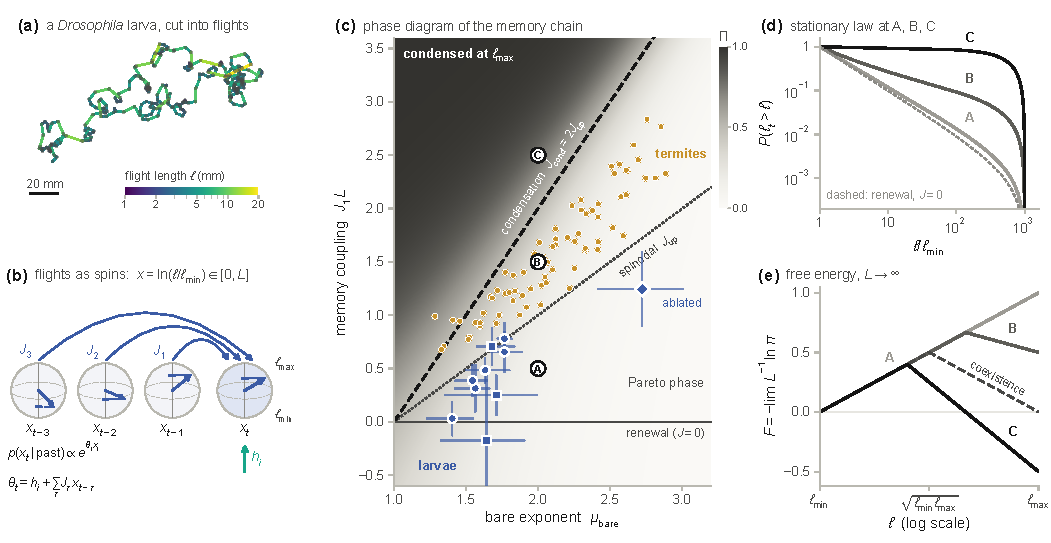
\includegraphics[width=\textwidth]{figs/fig1_overview.pdf}
\caption{From a track to a chain of spins. (a)~One hour of a \emph{Drosophila} larva (shi/+, 33\,$^\circ$C) crawling on plain agar: the flights (black segments, dots at the turns) cut out of the recorded track (grey). (b)~In the variable $x=\ln(\ell/\lmin)\in[0,L]$ a flight is the vertical projection of a classical spin on a sphere whose poles are the cutoffs $\lmin$ and $\lmax$; shown are four consecutive flights of the larva in (a). The next flight $x_t$ feels a field $h_i$, specific to the walker, and the previous flights through the couplings $J_\tau$, Eq.~\eqref{eq:causal}. (c)~Phase diagram of the chain with one lag, in the plane of the bare exponent $\mub=1-h$ and of the coupling $J_1L$. Shading: fraction $\Pi$ of flights longer than $\sqrt{\lmin\lmax}$ for $\lmax/\lmin=10^2$. Dotted, the spinodal $J=\Jup$; dashed, the self-dual condensation line $J=\Jcond=2\Jup$, Eq.~\eqref{eq:thresholds}. Indigo: larval conditions (median and interquartile range of $\mub$ over larvae, $\pm2$ s.e.\ of $J_1L$; circles, controls; squares, neurons silenced; diamond, brain lobes and sensory neurons ablated); ochre: 75 termite workers (Sec.~\ref{sec:data}). (d)~Stationary distribution of flight lengths at the states A, B and C marked in (c), for $\lmax/\lmin=10^3$; dashed, the renewal walk with the same $\mub$. (e)~Free energy $F(u)=-\lim_{L\to\infty}L^{-1}\ln\pi$ along $u=\ln(\ell/\lmin)/L$, Eq.~\eqref{eq:freeenergy}. It is piecewise linear because the stationary weight is a product of exponentials in $x$. In A the only minimum is at $\lmin$; in B a second, higher minimum at $\lmax$ makes runs of long flights metastable; on the dashed coexistence line the two minima are degenerate; in C the flights condense at $\lmax$.}
\label{fig:overview}
\end{figure*}

\subsection{One flight}\label{sec:single}

A flight length has no natural unit, so we measure it on a logarithmic scale. Every data set also comes with two bounds: a shortest flight $\lmin$, set by the resolution of the measurement, and a longest one $\lmax$, set by the walker, by the arena or by the duration of the recording. We keep both from the start and work with
\begin{equation}
x=\ln\frac{\ell}{\lmin}\in[0,L],\qquad L=\ln\frac{\lmax}{\lmin},
\label{eq:x}
\end{equation}
so that $L$ counts the $e$-folds spanned by the flights, between 3 and 6 for the walkers of Sec.~\ref{sec:data}. The measure $dx=d\ell/\ell$ is the only one that a change of units leaves invariant, up to a shift of $x$. Maximizing the entropy $S[p]=-\int_0^Ldx\,p(x)\ln p(x)$ at fixed $\langle x\rangle$ gives
\begin{equation}
p(x)=\frac{e^{\theta x}}{Z(\theta)},\qquad Z(\theta)=\frac{e^{\theta L}-1}{\theta},
\label{eq:single}
\end{equation}
which is a power law $p(\ell)\propto\ell^{-\mu}$ truncated to $[\lmin,\lmax]$, with $\mu=1-\theta$~\cite{Montroll1983}. (A MaxEnt law of flight lengths is thus a Pareto law; a L\'evy-stable law describes instead the sum of many flights.)

For a single flight, $\lmax$ is a convenience. On the half-line $x\ge0$, Eq.~\eqref{eq:single} is a normalized law whenever $\theta<0$, that is, $\mu>1$, and one may let $\lmax\to\infty$. The cutoff does make room for the opposite case: on $[0,L]$ any $\theta$ is allowed, and $\theta>0$ describes a walker whose flights pile up near $\lmax$. Section~\ref{sec:path} shows that, once flights remember each other, this case cannot be avoided, and the cutoff becomes a necessity.

The mean and the variance of $x$ are
\begin{equation}
\begin{aligned}
\langle x\rangle&=\Lambda(\theta)\equiv\frac L2\Big[1+\Lang\Big(\frac{\theta L}2\Big)\Big],\\
\mathrm{Var}\,x&=\Lambda'(\theta)=\frac{L^2}{4}\,\Lang'\Big(\frac{\theta L}2\Big),
\end{aligned}
\label{eq:langevin}
\end{equation}
where $\Lang(y)=\coth y-1/y$ is the Langevin function of paramagnetism [\figref{fig:theory}(a)]. Its appearance has a simple explanation. In the variable $u=2x/L-1\in[-1,1]$ the law~\eqref{eq:single} reads $p(u)\propto e^{bu}$ with $b=\theta L/2$. This is exactly the law of the vertical component $u=\cos\vartheta$ of a classical Heisenberg spin, a unit vector in three dimensions, in a field $b$: the area of a sphere between two heights is proportional to the distance between them (Archimedes' hat-box theorem), so $\cos\vartheta$ is uniform on $[-1,1]$ for a spin without field, and the Boltzmann factor $e^{b\cos\vartheta}$ tilts it as $e^{\theta x}$ tilts the flight. A flight is therefore a paramagnetic spin, which points to the south pole when the flight is close to $\lmin$ and to the north pole when it is close to $\lmax$ [\figref{fig:overview}(b)], and $\langle u\rangle=\Lang(b)$ is its magnetization. For the planar spins that describe directions of motion in Ref.~\cite{Agliari2024}, the Bessel ratio $I_1/I_0$ plays the same role. The susceptibility $\Lambda'$ is largest at $\theta=0$, where the histogram of $\ln\ell$ is flat and $\Lambda'(0)=L^2/12$; this number will set the critical point of the collective speed in Sec.~\ref{sec:meanfield}.

\subsection{A sequence of flights}\label{sec:path}

A walker produces flights $\mathbf x=(x_1,\dots,x_T)$ one after the other [\figref{fig:overview}(a)]. Following Ref.~\cite{Agliari2024}, in the spirit of maximum caliber~\cite{Presse2013}, we maximize the entropy of the whole sequence, $S[P]=-\int\mathcal Dx\,P[\mathbf x]\ln P[\mathbf x]$ with $\mathcal Dx=\prod_tdx_t$, at fixed mean of $x$ and fixed lagged correlations
\begin{equation}
C(\tau)=\frac1{T-K}\sum_{t=K+1}^T\langle x_tx_{t-\tau}\rangle,\qquad\tau=1,\dots,K .
\end{equation}
With Lagrange multipliers $h$ and $J_\tau$,
\begin{equation}
P[\mathbf x]=\frac1{Z_T}\exp\Big[\sum_tx_t\Big(h+\sum_{\tau=1}^KJ_\tau\,x_{t-\tau}\Big)\Big],
\label{eq:joint}
\end{equation}
the Boltzmann weight of a one-dimensional chain of continuous spins in time, in a field $h$ and with couplings $J_\tau$ of range $K$ [\figref{fig:overview}(b)]. For $K=0$ the flights are independent and identically distributed: this is the renewal L\'evy walk. A positive coupling means that long flights tend to follow long flights, a negative one that they alternate with short ones. With Gaussian instead of scale-free constraints the same construction gives Burg's maximum-entropy autoregression~\cite{Burg1975,CoverThomas}.

This is where the upper cutoff earns its place. Seen from flight $t$, the past acts as an effective field $h+\sum_\tau J_\tau x_{t-\tau}$. With $J_\tau>0$ this field grows with the length of the previous flights and, after long enough ones, becomes positive. On the half-line there is no normalizable law $e^{\theta x}$ with $\theta>0$, and the weight~\eqref{eq:joint} itself cannot be normalized. On $[0,L]$ every history yields a proper law, and every value of the parameters is allowed. What the cutoff costs is a scale: the largest change of field that one flight can produce on another is $J_\tau L$, and it is this product, not $J_\tau$ alone, that measures the strength of the memory (Sec.~\ref{sec:condensation}).

When several walkers are observed together, we give each walker $i$ its own field $h_i$. The fields absorb the differences between individuals, a quenched random field in the language of disordered systems, while the couplings, which describe the memory, are shared.

\subsection{The causal chain}\label{sec:causal}

The normalization $Z_T$ couples all the flights of Eq.~\eqref{eq:joint}, which makes its likelihood costly to evaluate. Agliari \emph{et al.} removed the difficulty with a mean-field step~\cite{Agliari2024}: in the weight of each spin they replaced the field generated by the past with the value it takes on the observed data, and normalized spin by spin, which makes the measure factorize in time. For one walker this step has an exact meaning. Each factor becomes the law of the next flight given the observed previous ones,
\begin{equation}
p(x_t\,|\,x_{t-1},\dots,x_{t-K})=\frac{e^{\theta_tx_t}}{Z(\theta_t)},\qquad
\theta_t=h+\sum_{\tau=1}^KJ_\tau\,x_{t-\tau},
\label{eq:causal}
\end{equation}
and their product is the probability of the observed sequence under a Markov chain of order $K$. This chain is a MaxEnt object in its own right: it maximizes the causal entropy $\sum_tH(x_t\,|\,x_{t-1},\dots,x_{t-K})$ under the same constraints~\cite{Ziebart2013}, and it is the model we use. At each turn the walker draws a truncated power law whose exponent, $\mu_t=1-\theta_t$, is set by its recent flights.

The log-likelihood
\begin{equation}
l(h,\bm J)=\sum_t\big[\theta_tx_t-\ln Z(\theta_t)\big]
\label{eq:loglik}
\end{equation}
is an elementary function of the parameters, and it is concave, because $\ln Z$ is convex and $\theta_t$ is linear in $(h,\bm J)$. Its maximum, when it exists, is unique. The stationarity conditions,
\begin{equation}
\sum_t\big[x_t-\Lambda(\theta_t)\big]=0,\qquad\sum_t\big[x_t-\Lambda(\theta_t)\big]\,x_{t-\tau}=0,
\label{eq:score}
\end{equation}
are the dynamic version of moment matching: the difference between each flight and its predicted mean must vanish on average and be uncorrelated with the past. The Fisher information,
\begin{equation}
\mathsf I=\sum_t\Lambda'(\theta_t)\,\bm z_t\bm z_t^{\mathsf T},\qquad \bm z_t=(1,x_{t-1},\dots,x_{t-K}),
\label{eq:fisher}
\end{equation}
gives the error bars. No Gaussian surrogate of the likelihood is needed: Eq.~\eqref{eq:loglik} is maximized as it is.

The path measure~\eqref{eq:joint} and the causal chain~\eqref{eq:causal} are different families with the same sufficient statistics. They agree to first order in $J$, after a shift of the field, and fitted to the same flights they return nearly the same couplings (Appendix~\ref{app:single}). In both, the selected depth is a Markov order~\cite{Ge2012}: $K^*=0$ is renewal, $K^*=1$ a Markov chain of flights, $K^*>1$ a longer memory. We call
\begin{equation}
\mub=1-h
\end{equation}
the bare exponent, the exponent of the next flight after a run of the shortest ones ($x_{t-\tau}=0$). With memory it differs from the exponent of the histogram of all flights (Sec.~\ref{sec:dressing}).

\begin{figure*}[t]
\centering
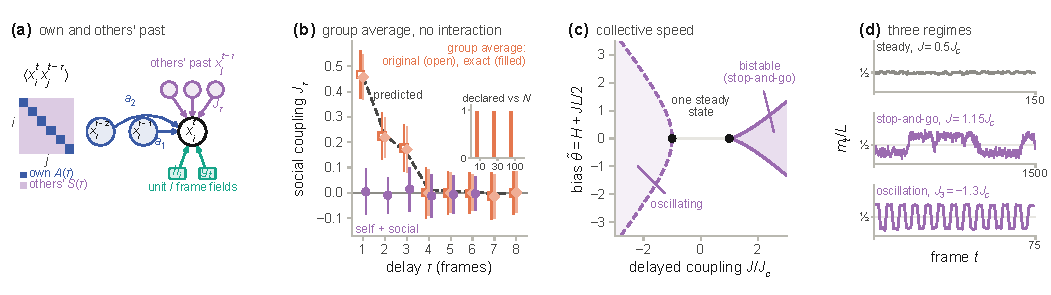
\includegraphics[width=\textwidth]{figs/fig2_many.pdf}
\caption{Many walkers. (a)~The lagged correlation between units has a diagonal part, each unit with its own past ($A$), and an off-diagonal part, each unit with the others' past ($S$); the group average mixes the two, Eq.~\eqref{eq:Rsplit}. The self\,+\,social model~\eqref{eq:selfsocial} gives each part its own couplings, $a_\tau$ and $J_\tau$, and adds a field for each unit, $h_i$, and for each frame, $g_t$. (b)~Synthetic units with own memory of depth 3 and no interaction ($N=30$, 40 replicates, mean $\pm$ s.d.): couplings returned by the group-average analysis in its original implementation (open squares) and with its exact likelihood (filled diamonds), against the prediction of Eq.~\eqref{eq:aggregation} (dashed); circles, social couplings of the self\,+\,social model. Inset: fraction of data sets in which a social coupling is declared, for $N=10$, 30 and 100. (c)~Mean-field phase diagram of the collective speed with one delayed coupling $J$, in units of $J_c=12/L^2$, and bias $\tilde\theta$: two stable states (shaded, solid boundary) for $J>J_c$, oscillations (dashed boundary) for $J<-J_c$; dots, the critical points. (d)~Group average on the symmetric line $\tilde\theta=0$: one steady state ($J=0.5J_c$, $N=200$), collective stop-and-go ($J=1.15J_c$, $N=40$), and oscillations of period 6 for a negative coupling at delay 3 ($N=200$). $L=\ln100$ throughout.}
\label{fig:many}
\end{figure*}

\subsection{Many walkers on a common clock}\label{sec:many}

In a group, the flights of different individuals start and end at different times, so ``the previous flight of the others'' is not defined. A group needs a common clock. We use frames $t$ of fixed duration and, for unit $i$, the log-displacement per frame, or log-speed, $x_i^t=\ln(\ell_i^t/\lmin)\in[0,L]$, with the same single-site law~\eqref{eq:single}.

Frames and flights are two different observables, and they answer different questions. On a frame clock a single flight spans many frames, so a walker's memory from one frame to the next mostly measures how long it keeps moving fast or slow; a renewal L\'evy walk observed in frames is strongly correlated, simply because its flights last. Whether a walker is a renewal process can only be asked of its flights, the events at which it chooses anew, and that is what we do for single walkers. Whether a walker responds to the others can only be asked on a common clock, and that is what we do for groups. The model is the same; only the index of time changes.

Transcribing Eq.~(A16) of Ref.~\cite{Agliari2024} from directions to log-speeds gives the path measure
\begin{equation}
P(\mathbf x)=\frac1Z\exp\Big[\sum_{t,i}x_i^t\Big(H+\frac1N\sum_{\tau=1}^{\tau_M}J_\tau\sum_jx_j^{t-\tau}\Big)\Big],
\label{eq:pre}
\end{equation}
which fixes the mean of $x$ and the lagged autocorrelation $R(\tau)=\langle m_tm_{t-\tau}\rangle$ of the group average $m_t=N^{-1}\sum_ix_i^t$. This autocorrelation contains two different things,
\begin{equation}
R(\tau)=\frac1NA(\tau)+\Big(1-\frac1N\Big)S(\tau),
\label{eq:Rsplit}
\end{equation}
where $A(\tau)$ is the mean lagged correlation of each unit with its own past and $S(\tau)$ that with the past of the others [\figref{fig:many}(a)]. In Eq.~\eqref{eq:pre} one multiplier $J_\tau$ accounts for both. Giving each its own multiplier, and each unit and each frame its own field, yields the self\,+\,social model,
\begin{equation}
\theta_i^t=h_i+g_t+\sum_{\tau=1}^{K_s}a_\tau\,x_i^{t-\tau}+\sum_{\tau=1}^{K_c}J_\tau\,s_i^{t-\tau},
\label{eq:selfsocial}
\end{equation}
with $p(x_i^t\,|\,\text{past})=e^{\theta_i^tx_i^t}/Z(\theta_i^t)$ and units independent of each other given the past of all. The self couplings $a_\tau$ are the memory of Sec.~\ref{sec:causal}. The social couplings $J_\tau$ act on $s_i^{t-\tau}$, the mean log-speed at frame $t-\tau$ of all other units (global coupling) or of the $k$ units nearest to $i$ (local coupling). The time fields $g_t$ absorb whatever affects all units at once. The model of Ref.~\cite{Agliari2024} is the special case $h_i=H$, $g_t=0$, $a_\tau=J_\tau/N$, $s=m$.

In Eq.~\eqref{eq:selfsocial} a unit's own past and the past of its neighbors enter in exactly the same way, as a field on its next step weighted by a coupling. Formally, the unit's own previous step is one more neighbor, the one that is always at distance zero: a memory is an interaction with one's own past, and an interaction is a memory of somebody else's. The two differ in what can produce them. Own memory can come from inertia, physiology or the persistence of a behavioral state; a coupling to the others' past requires that the unit perceives them, or that something drives both. They are kept in separate terms because the data offer them separately, in the diagonal and off-diagonal blocks of the lagged correlations of Fig.~\ref{fig:many}(a). For the same reason the single-walker model is not the trivial case $N=1$ of the collective one: it is the diagonal term that must be modeled before the off-diagonal one can be read.

% =============================================================================
\section{Physics of the memory chain}\label{sec:statmech}

\subsection{The stationary law}\label{sec:stationary}

With one lag, $\theta(x)=h+Jx$, the causal chain~\eqref{eq:causal} satisfies detailed balance with respect to
\begin{equation}
\pi(x)\propto e^{hx}\,Z(h+Jx),\qquad \pi(x)\,p(y\,|\,x)\propto e^{h(x+y)+Jxy},
\label{eq:stationary}
\end{equation}
as one checks by inserting Eq.~\eqref{eq:single} (Appendix~\ref{app:single}). The joint law of two consecutive flights is a two-site Boltzmann weight of Ising type, with continuous spins on $[0,L]$, and every stationary property of the walk follows from it.

The stationary law has a simple reading. In a reversible chain, the weight of a flight $x$ is the total weight of the pairs it forms with its successor, $\int_0^Ldy\,e^{h(x+y)+Jxy}=e^{hx}Z(h+Jx)$. The first factor is the bare power law. The second counts the successors: for $J>0$ a long flight forms favorable pairs with long successors, so the factor $Z(h+Jx)$ grows with $x$, roughly as $e^{JxL}$ once the field $h+Jx$ is positive, and it lifts the tail of the distribution. Figure~\ref{fig:overview}(d) shows the effect at the three states marked in the phase diagram of \figref{fig:overview}(c), all with the same bare exponent. In A, a weak coupling, the stationary law is barely distinguishable from the renewal one; in B the tail bends upward before the cutoff; in C most flights sit at $\lmax$.

\subsection{Duality and condensation}\label{sec:condensation}

Exchange long and short flights, $\ell\to\lmin\lmax/\ell$, that is, $x\to L-x$. For a renewal walker this maps the exponent $\mu$ onto $2-\mu$, a law that favors short flights onto one that favors long ones. With memory, the pair weight $e^{h(x+y)+Jxy}$ keeps its form: the coupling is unchanged and the field becomes $-h-JL$, up to a constant. A chain at $(h,J)$ and one at $(-h-JL,J)$ are thus the same chain read upside down, and the inversion is a duality. The chains with $h=-JL/2$ are mapped onto themselves. Their stationary law is symmetric under inversion, so exactly half of their flights are longer than the geometric mean $\sqrt{\lmin\lmax}$. With $\mub=1-h$, the self-dual line is the coupling
\begin{equation}
\Jcond=\frac{2(\mub-1)}{L}=2\Jup,\qquad \Jup=\frac{\mub-1}{L}.
\label{eq:thresholds}
\end{equation}

Both thresholds have a direct meaning. Take $\mub>1$, a rule that by itself favors short flights. After a flight at the cutoff, $x=L$, the field is $h+JL=JL-(\mub-1)$, and it is positive, so that the next flight is more likely long than short, when $J>\Jup$. Above this coupling a run of long flights can sustain itself. Whether the walker spends most of its time in such runs is decided by the duality: below $\Jcond$ it lives among short flights, above it among long ones. The fraction $\Pi$ of flights longer than $\sqrt{\lmin\lmax}$ is therefore the natural order parameter, and
\begin{equation}
\Phi=\frac J\Jup=\frac{JL}{\mub-1}
\end{equation}
the natural control parameter, with $\Phi=1$ at the first threshold and $\Phi=2$ at the second.

For wide ranges the change becomes a sharp transition. Since $\ln Z(\theta)=L\max(\theta,0)+O(\ln L)$, at fixed $\alpha=\mub-1>0$ and $\beta=JL$ the stationary law obeys a large-deviation principle in $L$,
\begin{equation}
\pi(x)\asymp e^{-L\,F(x/L)},\qquad F(u)=\alpha u-\max(\beta u-\alpha,0),
\label{eq:freeenergy}
\end{equation}
with $u=x/L\in[0,1]$ [\figref{fig:overview}(e)]. The logarithmic range $L$ plays the role of system size and $F$ that of a free energy per unit size. Because both factors of $\pi$ are exponentials in $x$, $F$ is piecewise linear and its minima can only sit at the ends, $u=0$ (flights near $\lmin$) and $u=1$ (flights near $\lmax$). For $\beta<2\alpha$ the global minimum is $u=0$ and $\Pi\to0$: the walker is in a Pareto phase, with a power-law histogram. For $\beta>2\alpha$ the global minimum is $u=1$ and $\Pi\to1$: the flights condense at the cutoff. The transition, on the self-dual line, is first order, with $\Pi$ jumping from 0 to 1. Between the two thresholds, $\alpha<\beta<2\alpha$, the end $u=1$ is a local minimum: a run of flights near $\lmax$ is metastable, and it lasts for a number of flights that grows exponentially with $L$ (Appendix~\ref{app:largeL}); $J=\Jup$ is the spinodal. At finite $L$ the jump is smoothed over a width of order $1/L$, and the curves $\Pi(\Phi)$ for different ranges cross at the self-dual point $\Phi=2$, $\Pi=1/2$ [\figref{fig:theory}(b)], as observables do at first-order transitions in finite systems~\cite{BinderLandau1984}.

Both thresholds vanish as $\lmax/\lmin\to\infty$. This reflects how the coupling scales, not a pathology. The coupling acts through $JL$, the largest change of field that one flight can impose on the next, and it is $JL$ that must be held fixed as the range grows, much as the couplings of a mean-field magnet must scale with the inverse number of spins. At fixed $J$ a wider range makes the same coupling stronger, and on the half-line every positive coupling lies beyond condensation, which is another way of saying that the chain does not exist there. At fixed $\Phi$ the limit $L\to\infty$ is well defined, and it is the limit in which the transition becomes sharp. The cutoff is therefore a physical ingredient of a L\'evy walk with memory, not a regularization to be removed at the end. Real data span one to two and a half decades, where the transition is a broad crossover, but its location still organizes the phase diagram in which the walkers of Sec.~\ref{sec:data} sit [\figref{fig:overview}(c)].

\subsection{Memory dresses the exponent}\label{sec:dressing}

A histogram does not know in which order the flights came. An i.i.d.\ truncated-Pareto fit to stationary flights matches their mean log length and returns $\hat\mu=1-\Lambda^{-1}(\langle x\rangle_\pi)$. For $J>0$ this exponent is smaller than $\mub$ [\figref{fig:theory}(c)]: memory packs long flights into runs, the histogram is heavier-tailed than the rule that generates it, and a walker with memory looks more L\'evy than its one-step rule. On the self-dual line $\langle x\rangle_\pi=L/2$ and $\hat\mu=1$ exactly, for every range. Put differently, the local exponent $\mu_t=1-\theta_t$ fluctuates with the recent past, a superstatistics~\cite{BeckCohen2003} generated by the dynamics itself. The exponent of a histogram is thus not a property of the search rule alone; it also depends on the memory and on the range over which it is measured. In real walkers the difference exceeds half a unit (Sec.~\ref{sec:data}).

\subsection{A critical point for the collective speed}\label{sec:meanfield}

Groups raise a question that single walkers do not: can a delayed coupling between walkers order the group as a whole? Take $N$ units with a global delayed coupling and no own memory, that is, Eq.~\eqref{eq:selfsocial} with $a_\tau=0$, $s_i$ the mean of all other units, a common field $h_i=H$ and no time fields. The group average $m_t$ plays the role of a magnetization. It is the collective log-speed, close to $0$ when the whole group crawls and close to $L$ when it runs. Two parameters control it. One is the total coupling $J_{\rm tot}=\sum_\tau J_\tau$, the strength with which the past speed of the group feeds back on its present. The other is a bias. Exchanging slow and fast, $m\to L-m$, maps the model onto itself with $H\to-H-J_{\rm tot}L$, the duality of Sec.~\ref{sec:condensation} at the level of the group; its symmetric point is $H=-J_{\rm tot}L/2$, and
\begin{equation}
\tilde\theta=H+\frac{J_{\rm tot}L}2
\end{equation}
measures the distance from it, positive when the group is biased toward running.

For $N\to\infty$ the units are independent given the past, and $m_t$ follows the deterministic delayed map
\begin{equation}
m_t=\Lambda\Big(H+\sum_\tau J_\tau m_{t-\tau}\Big),
\label{eq:map}
\end{equation}
with $\Lambda$ the Langevin response~\eqref{eq:langevin}. A steady state $m^*$, with field $\theta^*$, loses stability when a root $z$ of $1=\Lambda'(\theta^*)\sum_\tau J_\tau z^{-\tau}$ crosses the unit circle (Appendix~\ref{app:collective}). For positive couplings the first root to cross is $z=1$, a fold at which a second stable state appears. Since the susceptibility of one flight never exceeds $L^2/12$ (Sec.~\ref{sec:single}), this requires
\begin{equation}
J_{\rm tot}>J_c=\frac{12}{L^2},
\label{eq:Jc}
\end{equation}
with a cusp at $J_{\rm tot}=J_c$, $\tilde\theta=0$ [\figref{fig:many}(c)]. Above $J_c$ the group switches at random between a slow and a fast state, a collective stop-and-go whose residence times grow with $N$ [\figref{fig:many}(d)]. A negative coupling at delay $d$ makes the group oscillate instead: the map splits into $d$ independent sub-chains, each of which undergoes a period doubling at $|J|=J_c$, and any lag-1 inertia puts them in phase, so that the period is $2d$. Near both thresholds the fluctuations of the group average diverge, $N\,\mathrm{Var}(m)\to\Lambda'/[1-(\Lambda'J)^2]$ for one lag.

Own memory adds to the social feedback. With a lag-1 self coupling $a\ge0$, each unit at a steady state is the chain of Eq.~\eqref{eq:stationary} in the field $H+J_{\rm tot}m^*$, and the steady state loses stability when $J_{\rm tot}\chi=1$, where $\chi=\sum_{s\ge0}R(s)$ is the integrated response of one unit to a pulse of field. What enters is the response, not the integrated autocorrelation, which is 50\% larger at $a=0.2$. For $L=\ln100$ and $a=0.2$ the threshold drops to $J_c(a)=0.71J_c$, against $0.65J_c$ from the naive estimate $\Lambda'(0)(a+J)=1$, and the theory reproduces the simulated fluctuations within 1\% away from the threshold and within 4\% at $J=0.6J_c$ [Appendix~\ref{app:collective}, \figref{fig:collective}(b)].

The threshold $J_c=12/L^2$ exists because the support of each speed is compact, and it vanishes as the range grows. It is a scale-free and delayed counterpart of the speed criticality reported for starling flocks~\cite{Bialek2014}, where the interactions are instantaneous.

% =============================================================================
\section{From trajectories to couplings}\label{sec:inference}

\subsection{Fitting and choosing the depth}\label{sec:estimation}

For walkers $i=1,\dots,n$ with flights $x_{i,t}$, the field of Eq.~\eqref{eq:causal} becomes $\theta_{i,t}=h_i+\sum_\tau J_\tau x_{i,t-\tau}$, with one field per walker and shared couplings. The log-likelihood stays concave, and Newton's method finds its maximum in a few iterations (Appendix~\ref{app:estimation}). The cost is negligible. For one larval condition (6 to 59 larvae, 349 to 4240 flights) the whole scan of depths $K=0,\dots,6$, with one field per larva, takes 0.1--0.6\,s on a single core of a desktop computer; pooling all 241 larvae, with 241 fields and up to six couplings for 20\,948 flights, takes 5\,s. The same machinery accommodates fields that change every $B$ flights, which absorb slow drifts of the exponent and leave to the couplings only the short-range memory, and known covariates, such as the distance from a wall. Short tracks bias the couplings of a fit with one field per walker by an amount of order $1/T_i$~\cite{Nickell1981}, which we measure on surrogates in which the flights of each walker are permuted.

The depth is chosen by comparing models with $K=0,\dots,K_{\max}$, fitted on the same flights, through an information criterion, $\mathrm{AIC}=-2l+2k$ or $\mathrm{BIC}=-2l+k\ln n_{\rm o}$, with $k$ parameters and $n_{\rm o}$ predicted flights~\cite{Akaike1974,Schwarz1978}. The choice is not innocent. On renewal data AIC selects $K^*>0$ with asymptotic probability
\begin{equation}
P_{\rm AIC}=1-\exp\Big[-\sum_{k=1}^{K_{\max}}\frac1k\,P(\chi^2_k>2k)\Big],
\label{eq:woodroofe}
\end{equation}
equal to 0.248, 0.267, 0.284 and 0.288 for $K_{\max}=4$, 6, 12 and $\infty$, however long the data. This classical consequence of Spitzer's combinatorial lemma~\cite{Shibata1976,Woodroofe1982} makes AIC inconsistent for the order of a chain, and cross-validation with a fixed training fraction, asymptotically equivalent to it~\cite{Stone1977,Shao1993}, inherits the same bias. BIC is consistent~\cite{Katz1981,CsiszarShields2000}. Heavy tails play no role here, since in the log variable every sufficient statistic is bounded. We select the depth with BIC and calibrate every claim against surrogate data.

On walkers generated by the model itself with random parameters, the procedure does what it should (Appendix~\ref{app:selection}, \figref{fig:validation}). Planted and inferred couplings agree, and their differences, in units of the Fisher errors~\eqref{eq:fisher}, have mean $-0.01$ and standard deviation 0.97. BIC recovers the planted depth in 78\% of the walkers and never selects a deeper chain, whereas AIC does so in 24\%. On renewal walkers the false-positive rate of AIC stays at the level of Eq.~\eqref{eq:woodroofe} from 250 to 16\,000 flights, and that of BIC vanishes as the data grow.

\subsection{What else looks like memory}\label{sec:masquerade}

A real trajectory can mimic memory in ways that a planted walker cannot, and three of them matter here (Appendix~\ref{app:pitfalls}, \figref{fig:pitfalls}). Walkers differ: two flights of the same fast walker are both long, and a model with one field for all reads this as memory, at the largest depth allowed. One field per walker removes the effect, which is why we never pool walkers without their own fields. Flights are not observed but cut out of noisy tracks, and noise occasionally breaks a long flight into two long pieces, which manufactures a positive correlation; merging consecutive pieces that are nearly collinear undoes it, and a pipeline null, which rebuilds each track from its own flights in random order and analyzes it again, measures whatever memory the pipeline itself creates. Finally, the variable matters: the linear statistic $\ell_t\ell_{t-1}$ is dominated by a handful of extreme flights and misses a memory that the log statistic $x_tx_{t-1}$ detects. Different mechanisms of dependence also leave different signatures in how the selected depth grows with the length of the data, which helps to tell a finite memory from a slowly decaying one.

\subsection{Reading interactions from a group}\label{sec:groupavg}

For groups, three results, proved in Appendix~\ref{app:collective} and tested on synthetic collectives in Table~\ref{tab:collective}, organize the inference.

\emph{The mean-field measure is an exact likelihood.} The factorized measure of Ref.~\cite{Agliari2024}, evaluated on the data, equals the causal likelihood with $\theta_t=H+\sum_\tau J_\tau m_{t-\tau}$, as for single walkers in Sec.~\ref{sec:causal}. It can therefore be maximized exactly. The Gaussian autoregressive approximation used in the original implementation for convenience overestimates a planted coupling by 24\% in groups of five units; the exact estimator does not.

\emph{The group average contains own memory.} Let the units be independent, each with its own memory and autocovariance $C_i(\tau)$. A model of the group average then acquires delayed couplings, because the autocorrelation of the average contains the autocorrelation of each unit, Eq.~\eqref{eq:Rsplit}. Linearizing the inversion of Ref.~\cite{Agliari2024}, the fitted couplings converge to
\begin{equation}
\begin{gathered}
J^\star=\frac{\phi}{\Lambda'(\bar\theta)},\qquad\phi=\bar{\mathsf R}^{-1}\bar{\bm c},\\
\bar{\mathsf R}_{\tau\tau'}=\bar C(|\tau-\tau'|),\qquad \bar c_\tau=\bar C(\tau),
\end{gathered}
\label{eq:aggregation}
\end{equation}
the Yule--Walker coefficients of the mean individual autocovariance $\bar C=N^{-1}\sum_iC_i$, divided by the susceptibility of one unit. The factors of $N$ cancel, so these couplings do not shrink with the size of the group. In simulations without interactions the group-average analysis declares a delayed coupling in every data set, for $N=10$, 30 and 100 alike, with coefficients that follow Eq.~\eqref{eq:aggregation} lag by lag [\figref{fig:many}(b)]: $(0.468,0.225,0.177)$ against the predicted $(0.459,0.230,0.156)$ at $N=30$. These couplings are not an error of the analysis. They are the memories of the units, measured through their average, and a unit's own past is as legitimate a source of delayed correlation as the past of its neighbors; but the two are memories of a different nature, and the average cannot separate them. In the validation of Ref.~\cite{Agliari2024} on the Vicsek model, a peak at the first delay was correctly attributed to the inertia of each particle; Eq.~\eqref{eq:aggregation} shows that an inertia lasting longer than one frame produces peaks at longer delays as well. The self\,+\,social model assigns own memory to the couplings $a_\tau$: with regressors that leave out the unit itself, its social score vanishes exactly when units do not interact, and it declares a coupling in 1 of 120 interaction-free data sets.

\emph{Common drives look like interactions.} A field shared by all units, such as temperature, illumination or a pulse of chemokine, correlates units that never interact. Time fields $g_t$ absorb it, but they also absorb a global coupling: once each frame has its own field, the mean of the other units at an earlier frame is a function of that frame plus a multiple of the unit's own past, and global coupling and common drive become indistinguishable. A local coupling, which differs from unit to unit within a frame, survives. Local coupling with time fields is the only reading that declares no coupling under a drive alone and recovers a planted coupling without bias (Appendix~\ref{app:collective}, \figref{fig:collective}).

One last control is specific to real groups. In a time-shift surrogate each unit's track is displaced in time by an independent random offset. The surrogate keeps every unit's own memory, its heterogeneity and its marginal law, and it destroys every synchrony between units, both interactions and common drives. A coupling that survives in the surrogates is not an interaction.

% =============================================================================
\section{Walkers and groups in the data}\label{sec:data}

\begin{figure*}[t]
\centering
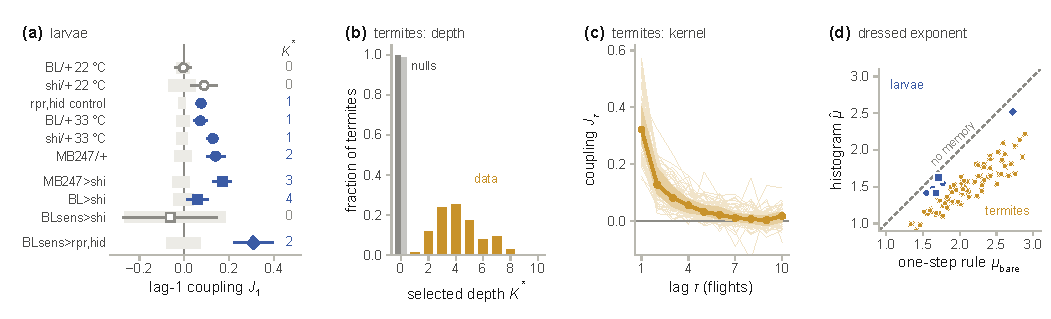
\includegraphics[width=\textwidth]{figs/fig3_walkers.pdf}
\caption{Single walkers. (a)~\emph{Drosophila} larvae: lag-1 coupling with one field per larva ($\pm2$ s.e.) and, on the right, the depth $K^*$ selected by BIC; filled symbols, $K^*>0$; grey bands, $\pm2$ s.d.\ over 30 within-larva permutations of the flights. Circles, controls; squares, neurons silenced with \emph{shibire}$^{ts}$; diamond, brain lobes and sensory neurons ablated (genotypes in Appendix~\ref{app:data}). (b)~Depth selected in each of 75 termites (ochre), and by the within-track permutation and pipeline nulls (grey), which select $K^*=0$. (c)~Memory kernel of the termites, from fits with $K=10$: single termites (thin lines), median and interquartile range. (d)~Exponent of the histogram of all flights, $\hat\mu$, against the exponent of the one-step rule, $\mub$, for the larval conditions with memory (medians over larvae, symbols as in (a)) and for each termite; dashed, the diagonal of renewal walkers.}
\label{fig:walkers}
\end{figure*}

All single walkers go through the same pipeline (Appendix~\ref{app:data}): flights are cut out of each track with a corridor of half-width $\varepsilon=0.5$\,mm, nearly collinear pieces are merged, $\lmin=1$\,mm, and $\lmax$ is the longest flight of the condition (larvae) or of the track (termites).

\subsection{\emph{Drosophila} larvae}\label{sec:larvae}

Sims \emph{et al.}~\cite{Sims2019} filmed \emph{Drosophila} larvae crawling for up to one hour on plain agar, without odor, light or food, and found L\'evy-like flight statistics that persisted when large parts of the nervous system were switched off. Neurons were targeted with the GAL4--UAS system. The driver BL expresses in the brain lobes and in part of the subesophageal ganglion, BLsens in the same regions and in all sensory neurons, MB247 in the mushroom bodies, a center of learning and memory. The targeted neurons were either silenced with \emph{shibire}$^{ts}$, a temperature-sensitive mutant of dynamin that blocks synaptic transmission above about 30\,$^\circ$C~\cite{Kitamoto2001} (the larvae were tested at 33\,$^\circ$C, some controls also at the permissive 22\,$^\circ$C), or killed by expressing the pro-apoptotic genes \emph{reaper} and \emph{hid} (\emph{rpr,hid}). Larvae that carry only the driver (BL/+, MB247/+) or only the effector (shi/+) are controls. Because the L\'evy statistics survived without brain and senses, Sims \emph{et al.} traced them to the central pattern generator for locomotion in the ventral nerve cord. In an environment controlled so tightly, these data are ideal to ask whether the intrinsic walk of the larva is a renewal process. The 241 tracks with at least 17 flights, 20\,948 flights in ten conditions, are fitted condition by condition with one field per larva and $K\le6$ (Table~\ref{tab:larvae}).

Renewal is rejected in seven of the ten conditions [\figref{fig:walkers}(a)]. The memory is positive, long flights tending to follow long flights, and short, one to four flights deep. It does not depend on how the flights are cut, and in six of the seven conditions it survives when the field of each larva is re-estimated every 25 flights, so it is not a slow drift of the exponent; in BL$>$shi it disappears, and is better described as a slow modulation (Appendix~\ref{app:data}). The nulls are clean: within-larva permutations select $K^*>0$ in 1 of 300 surrogates, and the pipeline null in none of 50. Of the three conditions compatible with renewal, BLsens$>$shi has too few flights (349) to decide, and shi/+ at 22\,$^\circ$C has a lag-1 coupling three standard errors from zero that BIC does not retain; only BL/+ at 22\,$^\circ$C shows no trace of memory.

The memory is strongest in the BLsens$>$\emph{rpr,hid} larvae, whose brain lobes and sensory neurons are dead: $J_1=0.31\pm0.05$, eight standard deviations from the permutation null. In the logic of Ref.~\cite{Sims2019}, the memory between flights is generated below the brain, together with the L\'evy-like statistics, and needs neither the brain nor sensory feedback.

Six of the seven conditions with memory sit at $\Phi\simeq0.7$--1.0 [\figref{fig:overview}(c)], close to the spinodal and about half way to condensation; BL$>$shi, whose memory is a slow modulation, sits at 0.35. Replacing the longest observed flight by the side or the diagonal of the $240\times240$\,mm arena changes $\Phi$ by at most 0.2, because $\mub$ and $J_1$ readjust with $L$. The exponent is visibly dressed [\figref{fig:walkers}(d)]: the one-step rule has $\mub=1.54$--1.77 (2.72 for the ablated larvae), the histogram $\hat\mu=1.41$--1.63 (2.52), and the stationary law of the fitted chains reproduces every observed $\hat\mu$ within 0.03. Over the full range of flights a truncated log-normal law describes the histogram better than a truncated power law in eight conditions out of ten, so ``L\'evy'' here means at most two decades of approximate scaling; the memory is the same with either single-flight law (Appendix~\ref{app:data}).

\subsection{Termites}\label{sec:termites}

Castiblanco \emph{et al.}~\cite{Castiblanco2019} tracked focal workers of the termite \emph{Cornitermes cumulans} for 6\,h at 2\,Hz, in Petri dishes about 49\,mm across, together with nestmates at different densities. Each of the 75 tracks contains 673 to 12\,091 flights (median 3746), enough to analyze every termite on its own, with $K\le10$.

Every termite remembers. BIC selects a depth between 1 and 8, with a median of 4 [\figref{fig:walkers}(b)], and the lag-1 coupling is positive in all 75 tracks, $J_1=0.34\pm0.10$ (mean $\pm$ s.d.\ over termites); the memory kernel decays over about five flights [\figref{fig:walkers}(c)]. Within-track permutations select memory in 0.3\% of the surrogates, and the pipeline null gives $K^*=0$ in 74 of 75 tracks. With fields re-estimated every 50 or 25 flights the lag-1 coupling stays significant in every termite (median $z=21$ and 18, minimum 6.3).

Termites, like many insects, keep close to walls, a behavior known as thigmotaxis: they spend 30\%, 59\% and 79\% of the time within 3, 6 and 9\,mm of the wall of the dish. The memory could therefore have been geometric, long flights along the wall following each other. It is not. Adding the wall state of each flight as a covariate leaves the lag-1 coupling unchanged (median 0.42 without and 0.41--0.43 with it, for the three bands) and the selected depth unchanged (median 4), and on runs of consecutive flights far from the wall the coupling is even larger, $J_1\simeq0.49$ (Appendix~\ref{app:data}).

The termites sit further into the phase diagram than the larvae, at $\Phi=1.0$--3.5 (median 1.46) [\figref{fig:overview}(c)]: all of them beyond the spinodal, and 7\% beyond the condensation line, consistent with an arena that bounds their longest flights. Their exponents are the most dressed [\figref{fig:walkers}(d)]. The one-step rule has a median $\mub=2.07$, the histogram $\hat\mu=1.49$: read from the histogram, the exponent is off by more than half a unit. The apparent exponent grows with the density of nestmates (medians 1.18, 1.51 and 1.59 at densities 0.08, 0.12 and 0.20).

\begin{figure*}[t]
\centering
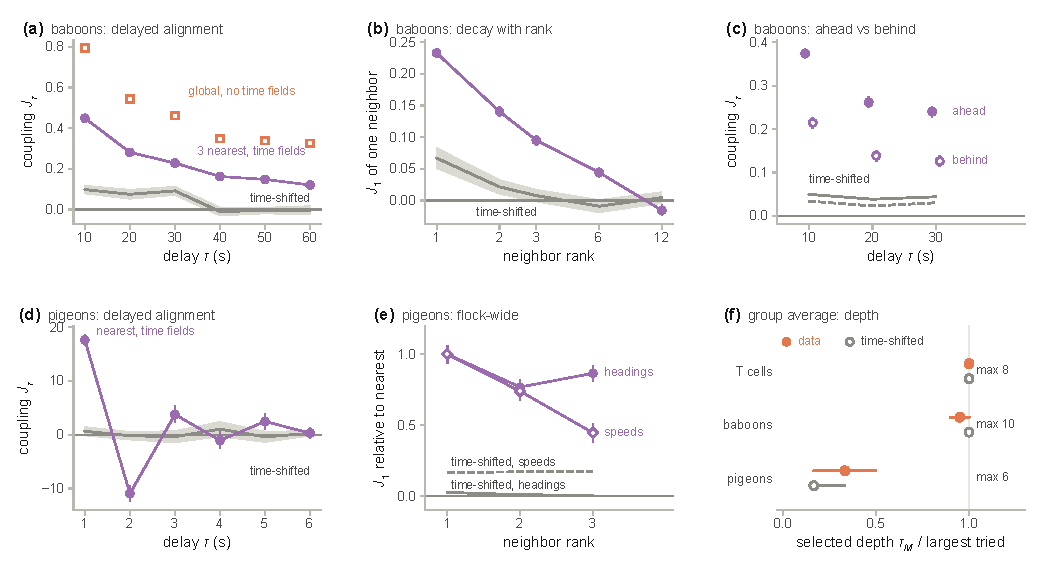
\includegraphics[width=\textwidth]{figs/fig4_groups.pdf}
\caption{Groups. Top: a wild baboon troop~\cite{StrandburgPeshkin2015} (14 days, clock 10\,s, headings). (a)~Couplings of a baboon's heading to the mean heading of its three nearest neighbors at delay $\tau$, with baboon and time fields ($\pm2$ s.e.); grey, mean $\pm2$ s.d.\ over 20 troops in which every baboon is shifted in time; open squares, a global coupling without time fields. (b)~Coupling at 10\,s to a single neighbor of given distance rank, all ranks fitted jointly. (c)~Couplings to the neighbors ahead (filled) and behind (open) along the group heading, among the six nearest; grey, time-shifted troops (solid, ahead; dashed, behind). Bottom: homing-pigeon flocks~\cite{MehlhausenFranks2025} (41 releases, clock 1\,s). (d)~As (a), for the nearest neighbor. (e)~Couplings at 1\,s to a single neighbor of given rank, relative to the nearest, for headings (filled) and log-speeds (open); grey, time-shifted flocks. (f)~Depth $\tau_M$ selected by the group-average analysis, as a fraction of the largest depth tried, on the data (coral) and on time-shifted units (grey): median and interquartile range over days (baboons), releases (pigeons) and surrogates; for the T cells, 16 fish pooled.}
\label{fig:groups}
\end{figure*}

\subsection{Baboons and pigeons}\label{sec:realgroups}

A wild troop of olive baboons~\cite{StrandburgPeshkin2015,Crofoot2015data}, 26 animals tracked by GPS every second for 14 days, is a group whose members share a clock and whose positions define neighbors. We use a clock of 10\,s, each day being a co-recorded group ($6\times10^4$ frames in all), and both variables, log-speeds and headings, a heading being defined for steps of at least 1\,m (Appendix~\ref{app:data}). Analyzed through its group average, the troop has a long memory: the selected depth has a median of 9.5 delays over days for headings and is 10, the largest tried, for log-speeds. Time-shifted baboons give the same depths, 10 in 82\% of the day replicates for headings and in all of them for log-speeds [\figref{fig:groups}(f)]. The depth is thus each baboon's own persistence ($\hat a_1=0.70$ for headings, 0.23 for log-speeds), seen through the average as in Eq.~\eqref{eq:aggregation}.

The self\,+\,social model, with baboon and time fields, finds in addition a delayed alignment with the three nearest neighbors, $J_1=0.449\pm0.007$ at 10\,s, which decays over a minute [\figref{fig:groups}(a)]; on a clock of 30\,s the first coupling is the same, $0.447\pm0.008$. Three controls single it out. Time-shifted baboons keep a coupling of $0.10\pm0.01$ at the shortest delays, because animals that pass the same place at different times head the same way, a field fixed in space that time fields cannot absorb; the data exceed it fourfold. The coupling lives at the nearest neighbors: $0.233\pm0.004$ with the single nearest, then 0.140, 0.095 and 0.044 with the second, third and sixth, and zero with the twelfth [\figref{fig:groups}(b)]. And it is asymmetric: neighbors ahead along the group heading weigh $0.374\pm0.006$, those behind $0.214\pm0.006$, against 0.050 and 0.034 for time-shifted baboons [\figref{fig:groups}(c)]. A baboon thus turns toward where its nearest neighbors, those ahead above all, were heading 10 to 30\,s earlier, in line with the following of initiators documented in this troop~\cite{StrandburgPeshkin2015}; a path walked first by those ahead would act in the same direction, and fields fixed in space would be needed to tell the two apart. Log-speeds tell the same story on a smaller scale, $J_1=0.052\pm0.002$ against $0.017\pm0.001$ for shifted baboons. Read with a global coupling and no time fields, the same headings give $J_1=0.79$ [\figref{fig:groups}(a), squares], the alignment plus the common motion of the troop.

Homing pigeons~\cite{MehlhausenFranks2025,MehlhausenFranks2025data}, three flocks released 41 times, form small groups of three to eight birds per frame, which we follow on a clock of 1\,s. On this scale flight is nearly ballistic, and a bird's heading is extrapolated from its last three, $\hat a_\tau=(185,-82,21)$, that is, from its direction and its rate of turn. The group-average analysis again returns the depths of time-shifted birds, 1 to 3\,s in 80\% of the releases against 91\% for shifted birds [\figref{fig:groups}(f)]. The self\,+\,social model couples each bird to its nearest neighbor with $J_\tau=(17.6\pm0.6,-11.0\pm0.8,3.8\pm0.8)$, against $(0.6\pm0.4,-0.2\pm0.4,-0.4\pm0.6)$ for shifted birds [\figref{fig:groups}(d)]. The alternating signs repeat those of own memory: a bird follows both the last heading of its neighbor and its last turn. In flocks this small the heading coupling does not decay over the three nearest neighbors, whereas speeds match the nearest one most [\figref{fig:groups}(e)]; log-speeds are coupled with $J_1=3.8\pm0.1$, against $0.5\pm0.2$ for shifted birds. Nor is the coupling stronger toward birds ahead ($3.5\pm0.3$ ahead, $5.3\pm0.3$ behind among the three nearest): pigeons follow their leaders with delays of fractions of a second~\cite{Nagy2010}, within one frame of this clock, and a model of delayed couplings sees only the interactions slower than its frame.

\subsection{A negative control: T cells}\label{sec:tcells}

T cells close the analysis as a negative control, first for single walkers. Jerison and Quake~\cite{Jerison2020} showed that the apparent heavy tails of their steps come from differences between cells, so any memory found with one field for all cells should be heterogeneity in disguise. It is. With one field for all cells, every group of T cells (and of \emph{Dictyostelium} amoebae from the same data set) shows deep memory, and it still does after the steps of each cell are shuffled ($K^*=5$--6 in 49 of 50 surrogates), which can only be heterogeneity. With one field per cell the shuffled data give $K^*=0$ in every surrogate, the memory of mouse T cells disappears, and zebrafish T cells and \emph{Dictyostelium} keep a short persistence ($J_1\simeq0.14$--0.15 per frame; Appendix~\ref{app:data}).

The same cells also test the group analysis. Zebrafish T cells co-recorded within each fish on a common clock of 45\,s (16 fish, 712 cells, 85\,016 steps) remember their own speed for about four frames ($\hat a_1\simeq0.20$). The group-average analysis selects a delay of 8 frames, the largest tried, and it selects the same delay in 20 of 20 time-shifted surrogates [\figref{fig:groups}(f)]: the delay is own memory. A weak coupling to the three nearest cells, $J_1=0.021\pm0.006$, vanishes once time fields are included, $0.005\pm0.007$; what remains is a drive shared within each fish. As far as the model can see, the cells do not interact.

The same model and the same controls thus return different answers for different groups: a delayed alignment of baboons with their nearest neighbors, stronger toward those ahead; a flock-wide coupling between pigeons, whose leader--follower delays are shorter than a frame; and no interaction between T cells. In none of the three could the answer be read off the group average, whose selected depth is in each case the own memory of the units.

% =============================================================================
\section{Discussion}\label{sec:discussion}

The renewal L\'evy walk is a convenient idealization, and most of the walkers analyzed here do not follow it. Larvae and termites remember their recent flights, positively and over a few flights, and the memory survives every control we could think of: one field per individual, fields that drift along the track, other ways of cutting tracks into flights, permutation and pipeline nulls, and, for the termites, the wall that they follow. In the larvae it is strongest when brain lobes and sensory neurons have been ablated, which places its origin, together with that of the L\'evy-like statistics~\cite{Sims2019}, below the brain. Part of the dependence between flights may come from switches between behavioral states, which a chain of flights describes as memory; couplings within each state would apportion the two~\cite{Stoye2025}.

Memory changes what a histogram means. A walker that packs long flights into runs has a heavier-tailed histogram than the rule it follows at each turn, by more than half a unit of exponent in the termites. An exponent read from a histogram, often compared with the value $\mu=2$ of optimal search~\cite{Viswanathan1999}, need not be the exponent of the rule that generates the walk. Memory also gives the cutoffs a physical role: the coupling acts through $JL$, the flights condense at the largest scale beyond a self-dual coupling, and over the one or two decades accessible to experiments the walk feels that transition well before reaching it: every termite has crossed its spinodal. Two extensions follow directly: a joint model of the length and the direction of flights, with couplings between speed and turning~\cite{Jerison2020}, and the transport properties of L\'evy walks whose flights are coupled in this way, to which renewal theory does not apply.

In groups, the same formalism separates what the group average mixes: each unit's memory of its own past, drives common to all units, and the influence of the others. Read through the average, own memory appears as a delayed coupling whose strength does not decrease with the size of the group, and a common drive as a coupling at any delay. Read with the self\,+\,social model, the delays found in zebrafish T cells are own memory and a drive shared within each fish, baboons align with where their nearest neighbors, those ahead above all, were heading 10 to 30\,s earlier, and pigeons are coupled to their whole flock from one second to the next. The recipe applies to any attempt to infer delayed interactions from trajectories: model units, not their average; give each unit its own field and memory and each frame its own field; couple units to their neighbors rather than to the group; compare with time-shifted units; and check how a coupling depends on the distance and on the position of the neighbor. Fields fixed in space, such as trails or a homing route, survive both time fields and time shifts, and are the natural next ingredient. Finally, the collective speed has a critical point of its own, at $J_c=12/L^2$, set by the largest susceptibility of a single flight: a delayed positive coupling between scale-free speeds produces collective stop-and-go, a negative one oscillations, and own memory lowers the threshold.


\section*{Data availability}
All trajectories analyzed in this work are publicly available~\cite{Sims2019,Castiblanco2019,Jerison2020,Crofoot2015data,MehlhausenFranks2025data}. The code that reproduces every analysis and figure will be made available upon publication.

\begin{acknowledgments}
We are grateful to the authors of Refs.~\cite{Sims2019,Castiblanco2019,Jerison2020,StrandburgPeshkin2015,MehlhausenFranks2025} for making their data public.
\end{acknowledgments}

\appendix
% =============================================================================
\section{One flight and the chain with one lag}\label{app:single}

\begin{figure*}[t]
\centering
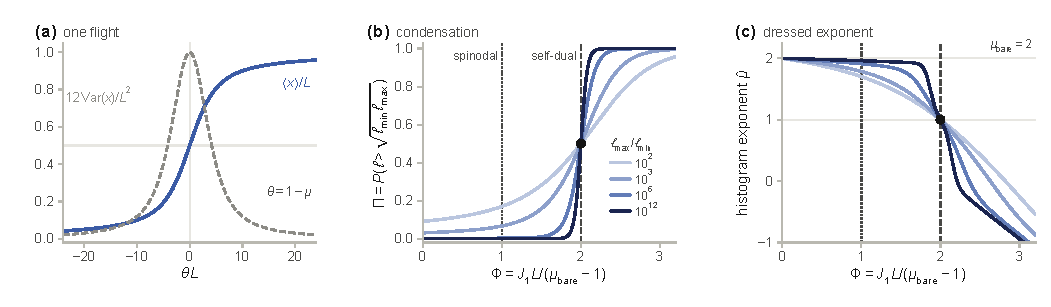
\includegraphics[width=\textwidth]{figs/figA1_theory.pdf}
\caption{The memory chain at depth one. (a)~Response of one flight to its field, Eq.~\eqref{eq:langevin}: mean (solid) and variance (dashed, in units of its maximum $L^2/12$) of $x$. (b)~Order parameter $\Pi$, the fraction of stationary flights longer than $\sqrt{\lmin\lmax}$, versus $\Phi=J_1L/(\mub-1)$ at $\mub=2$, for ranges $\lmax/\lmin$ from $10^2$ to $10^{12}$. The curves cross at the self-dual point $\Phi=2$, $\Pi=1/2$, and sharpen into a step as the range grows; dotted, the spinodal $\Phi=1$. (c)~Exponent returned by an i.i.d.\ truncated-Pareto fit to the same stationary laws: memory lowers it below $\mub$, and every curve crosses $\hat\mu=1$ at $\Phi=2$.}
\label{fig:theory}
\end{figure*}

\paragraph{Single-site law.} For $p(x)\propto e^{\theta x}$ on $[0,L]$, $Z(\theta)=(e^{\theta L}-1)/\theta$ and $\ln Z(\theta)=\theta L/2+\ln[2\sinh(\theta L/2)/\theta]$, so that
\begin{equation}
\frac{d\ln Z}{d\theta}=\frac L2+\frac L2\coth\frac{\theta L}2-\frac1\theta=\Lambda(\theta),\qquad \frac{d^2\ln Z}{d\theta^2}=\Lambda'(\theta),
\end{equation}
which is Eq.~\eqref{eq:langevin} [\figref{fig:theory}(a)]. With $u=2x/L-1$, $p(u)\propto e^{bu}$ on $[-1,1]$ with $b=\theta L/2$, and $\langle u\rangle=\Lang(b)$: this is the law of $\cos\vartheta$ for a classical unit vector with Boltzmann weight $e^{b\cos\vartheta}$, since the area element $\sin\vartheta\,d\vartheta\,d\varphi=-d(\cos\vartheta)\,d\varphi$ is uniform in $\cos\vartheta$. The maximum of $\Lambda'$ is at $\theta=0$, where $\Lang'(0)=1/3$ gives $\Lambda'(0)=L^2/12$. Adding the constraint $\langle x^2\rangle$ gives $p(x)\propto e^{\theta x-\beta x^2}$, a log-normal law truncated to $[\lmin,\lmax]$, which we use as a nested alternative, with integrals computed by Gauss--Legendre quadrature.

\paragraph{Detailed balance.} With $\pi(x)\propto e^{hx}Z(h+Jx)$ and the kernel $p(y|x)=e^{(h+Jx)y}/Z(h+Jx)$,
\begin{equation}
\pi(x)\,p(y|x)\propto e^{hx+(h+Jx)y}=e^{h(x+y)+Jxy},
\end{equation}
which is symmetric in $(x,y)$; $\pi$ is therefore stationary and the chain reversible. Under $x\to L-x$, $y\to L-y$ the exponent becomes $2hL+JL^2-(h+JL)(x+y)+Jxy$, the same weight with $h\to-h-JL$; the self-dual line is $h=-JL/2$.

\paragraph{Path versus causal measure.} The path measure~\eqref{eq:joint} with $K=1$ is a reversible Markov chain whose kernel is the Doob transform of its transfer operator, $p_{\rm path}(y|x)=e^{hy+Jxy}\varphi(y)/[\lambda_0\varphi(x)]$, with $\varphi$ the Perron eigenfunction of the kernel $e^{h(x+y)/2+Jxy}$ on $[0,L]$ and $\lambda_0$ its eigenvalue. The causal kernel is the same expression with $\varphi\equiv1$ and normalization $Z(h+Jx)$. Since $\ln\varphi(y)=J\langle x\rangle_0\,y+O(J^2)$, with $\langle x\rangle_0$ the mean at $J=0$, the two families coincide to first order in $J$ after the shift $h_{\rm causal}=h_{\rm path}+J\langle x\rangle_0$, and they differ at order $J^2$ through an effective log-normal curvature that grows near the thresholds. Fitted to $T=6000$ flights generated by either family, the two return $\hat J=0.095$ and 0.099, with log-likelihoods within 2 nats.

The path measure has the same duality, with self-dual line $h=-JL$ instead of $h=-JL/2$. In the path measure each flight interacts with both its neighbors in time, so a run of flights at the cutoff exerts on a flight a field $h+2JL$, against $h+JL$ in the causal chain, and the self-dual coupling is half as large at the same bare field. The two statements are not in conflict: the bare fields of the two families differ by $J\langle x\rangle_0$, so equal bare fields do not describe the same walk, and only the causal chain is used in this paper. We verified numerically, with the transfer operator on 160 Gauss--Legendre nodes, that on the self-dual line of the path measure $\Pi=1/2$ for every $L$, and that the crossover sharpens with $L$ as for the causal chain.

% -----------------------------------------------------------------------------
\section{Large-range theory of the condensation}\label{app:largeL}

For $\theta L\to+\infty$, $\ln Z(\theta)=\theta L-\ln\theta+o(1)$; for $\theta L\to-\infty$, $\ln Z(\theta)=-\ln|\theta|+o(1)$. With $h=-\alpha$, $J=\beta/L$ and $x=uL$, the field after a flight $x$ is $\theta=-\alpha+\beta u$, and
\begin{equation}
\ln\pi(uL)=-\alpha uL+L\max(\beta u-\alpha,0)+O(\ln L),
\end{equation}
which is Eq.~\eqref{eq:freeenergy}. $F(u)$ is piecewise linear: it increases with slope $\alpha$ for $u<\alpha/\beta$ and, if $\beta>\alpha$, decreases with slope $\alpha-\beta$ beyond. The end $u=1$ is thus a local minimum for $\beta>\alpha$ (spinodal, $J=\Jup$) and the global one for $\beta>2\alpha$ (coexistence, $J=\Jcond$), where $F(1)=2\alpha-\beta$ changes sign. The mass near each minimum is $e^{-LF}$ up to algebraic prefactors, so $\Pi\to\Theta(\beta-2\alpha)$ as $L\to\infty$, a first-order jump. At finite $L$ the exact condition for a secondary maximum of $\pi$ at the cutoff is $J\,\Lambda(h+JL)>\mub-1$, which tends to $J>\Jup$ for wide ranges; below $\Jcond$ its weight is exponentially small, $\pi(L)/\pi(0)\sim e^{(2h+JL)L}$.

Metastability can be seen directly. Starting a chain at $x=L$ in the window $\alpha<\beta<2\alpha$, the first flight shorter than $\sqrt{\lmin\lmax}$ occurs after a mean number of flights that grows exponentially with $L$: at $\beta=1.8\alpha$, from 4 at $\lmax/\lmin=10^2$ to 9 at $10^4$ and 73 at $10^8$ (4000 simulated chains each). In this window a walker that enters a run of long flights stays in it for a time set by the range, the dynamical signature of a metastable phase.

% -----------------------------------------------------------------------------
\section{Estimation}\label{app:estimation}

\paragraph{Likelihood and Newton's method.} Writing $\theta_{i,t}=\bm w\cdot\bm z_{i,t}$, with $\bm w$ collecting fields and couplings and $\bm z_{i,t}$ the corresponding regressors (indicators of the walker or block, lagged flights, covariates), the negative log-likelihood $-l=\sum_{i,t}[\ln Z(\theta_{i,t})-\theta_{i,t}x_{i,t}]$ has gradient $\sum[\Lambda(\theta)-x]\bm z$ and Hessian $\sum\Lambda'(\theta)\,\bm z\bm z^{\mathsf T}$, positive semi-definite. We use Newton's method with a backtracking line search, started from the renewal solution, which converges in a few iterations to a gradient below $10^{-8}$ per flight. The Hessian at the optimum is the observed Fisher information~\eqref{eq:fisher}; the sandwich covariance $\mathsf I^{-1}\mathsf G\,\mathsf I^{-1}$, with $\mathsf G$ the sum of outer products of the per-flight scores, guards against misspecification and is used for the couplings of the fits with one field per walker. All depths $K\le K_{\max}$ are fitted on the same flights, those with at least $K_{\max}$ predecessors, so that they can be compared. The timings quoted in Sec.~\ref{sec:estimation} use a dense Hessian on a single thread.

\paragraph{Centering and the bare exponent.} In the fits the lags are centered, $\theta_t=h+\sum_\tau J_\tau(x_{t-\tau}-c)$, with $c$ the mean of $x$ (of each track, with one field per walker), which decorrelates the field from the couplings. The bare exponent is $\mub=1-h'$, with $h'=h-c\sum_\tau J_\tau$ the field after a run of the shortest flights; its standard error follows from the delta method.

\paragraph{Fields per walker, local fields and covariates.} With one field per walker, $\bm z_{i,t}$ contains the indicator of walker $i$; with local fields, the indicator of the block of $B$ flights to which $t$ belongs (the last block is merged with the previous one if shorter than $B/2$); a known covariate $w_{i,t}$, such as the wall state of a flight, adds a column, $\theta_t\to\theta_t+g\,w_t$. The incidental-parameter bias of the couplings, of order $1/T_i$~\cite{Nickell1981}, is measured on surrogates in which the flights of each walker (or of each block) are permuted, and the $z$-scores of Table~\ref{tab:larvae} are computed against these permutation distributions.

% -----------------------------------------------------------------------------
\section{Model selection and validation}\label{app:selection}

\begin{figure*}[t]
\centering
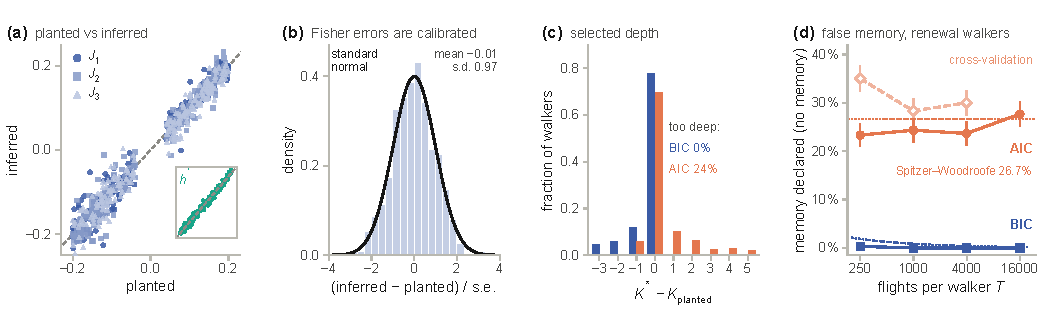
\includegraphics[width=\textwidth]{figs/figA2_validation.pdf}
\caption{Validation on planted walkers. (a)~Planted versus inferred couplings $J_1$, $J_2$, $J_3$ for 200 walkers of $T=3000$ flights, with bare exponents drawn uniformly in $[1.3,2.5]$, couplings of random sign and modulus in $[0.04,0.20]$, and $\lmax/\lmin=10^2$; inset: the field $h'=1-\mub$. (b)~Errors in units of the Fisher standard errors, pooled over all parameters, against the standard normal law. (c)~Selected depth minus planted depth: BIC never overestimates it, and underestimates it only when the last coupling is weaker than about three standard errors; AIC overestimates it in a quarter of the walkers. (d)~Fraction of renewal walkers ($\mub=2$, $\lmax/\lmin=10^3$, 300 replicates per length) declared to have memory by AIC, blocked cross-validation and BIC; dotted lines, the asymptotic values of Eq.~\eqref{eq:woodroofe} for AIC and $P(\chi^2_1>\ln T)$ for BIC.}
\label{fig:validation}
\end{figure*}

\paragraph{AIC and BIC under the null.} For nested models of depths $0,\dots,K_{\max}$, under the null the likelihood-ratio statistics of successive increments are asymptotically independent $\chi^2_1$ variables, so that $\Delta_k=\sum_{j\le k}(\chi^2_{1,j}-2)$ is a random walk with negative drift, and AIC selects the depth at which it is largest. Spitzer's combinatorial lemma gives the probability that the maximum is attained at $k=0$, hence Eq.~\eqref{eq:woodroofe}~\cite{Shibata1976,Woodroofe1982}. Replacing the penalty 2 by $\ln n_{\rm o}$ (BIC) makes the drift diverge, and the false-positive rate decreases as $P(\chi^2_1>\ln n_{\rm o})$ to leading order. Cross-validation with a fixed training fraction estimates the same expected out-of-sample log-likelihood as AIC and is asymptotically equivalent to it~\cite{Stone1977}; it becomes consistent only if the training fraction vanishes~\cite{Shao1993}. Our blocked cross-validation splits each track into five contiguous folds separated by gaps of $K_{\max}$ flights.

\paragraph{Planted walkers.} Walkers generated by the causal chain with random parameters (\figref{fig:validation}) lie along the diagonal of planted versus inferred couplings, and the errors in units of the Fisher standard errors have mean $-0.01$ and standard deviation 0.97. BIC recovers the planted depth in 78\% of the walkers and never selects a deeper one; when it errs, the last coupling is below detection. AIC selects a deeper chain in 24\% of the walkers. On renewal walkers the false-positive rate of AIC stays at the level of Eq.~\eqref{eq:woodroofe} for every length from 250 to 16\,000 flights, that of blocked cross-validation is slightly higher (28--35\%), and that of BIC vanishes as $P(\chi^2_1>\ln T)$. The rates are the same, 21--25\% for AIC and at most 0.5\% for BIC, for exponents $\mu=1.5$--2.5 and for ranges up to five decades.

% -----------------------------------------------------------------------------
\section{What can look like memory}\label{app:pitfalls}

\begin{figure*}[t]
\centering
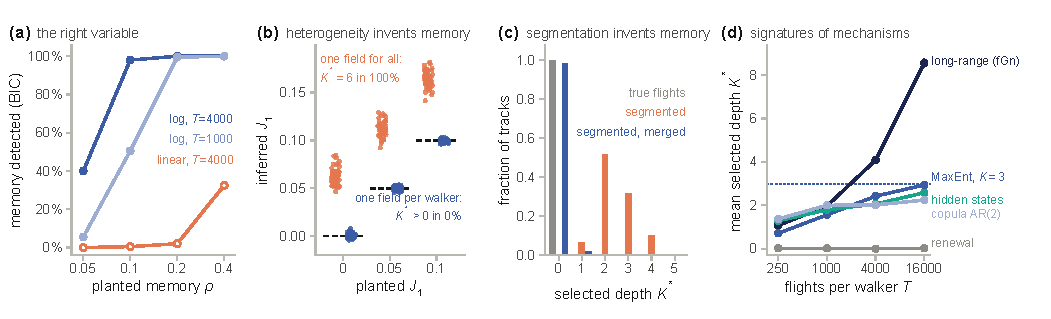
\includegraphics[width=\textwidth]{figs/figA3_pitfalls.pdf}
\caption{How memory is missed or invented, on synthetic walkers. (a)~Power to detect a weak memory with the log statistic $x_tx_{t-1}$ and with the linear statistic $\ell_t\ell_{t-1}$ (BIC; 200 replicates per point). (b)~Inferred lag-1 coupling for 40 walkers with individual exponents $\mu_i\sim U(1.2,2.2)$ and $T=1000$ flights each, with a common field (coral) or one field per walker (indigo); dashed, planted values. (c)~Selected depth for a renewal L\'evy walk sampled at fixed times with localization noise: true flights, flights segmented from the track, and segmented flights after merging nearly collinear pieces. (d)~Mean selected depth ($\pm$ s.e.) versus the number of flights for five mechanisms with truncated-Pareto marginals: renewal, a MaxEnt chain of depth 3 (dotted: its true depth), a Gaussian-copula AR(2) process, a walker switching between two hidden states, and long-range memory (Gaussian copula of fractional Gaussian noise with Hurst exponent 0.75).}
\label{fig:pitfalls}
\end{figure*}

\paragraph{The variable.} The statistic $\ell_t\ell_{t-1}$, the natural guess in linear space, is dominated by a handful of extreme flights. For a weak memory, a Gaussian-copula autoregression with truncated-Pareto marginals and correlation $\rho=0.1$ ($T=4000$), the log statistic $x_tx_{t-1}$ detects it in 98\% of the walkers and the linear one in none [\figref{fig:pitfalls}(a)].

\paragraph{Heterogeneity.} With 40 memoryless walkers whose exponents are spread over $[1.2,2.2]$, a model with a common field selects the maximal depth in every replicate and returns $J_1\simeq0.11$ for a planted $0.05$. One field per walker removes both the false positives and the bias [\figref{fig:pitfalls}(b)].

\paragraph{Corridor segmentation.} Positions are sampled at fixed times with noise, and flights must be cut out of the track. A flight is the longest stretch of track that stays within a corridor of half-width $\varepsilon$ around the segment joining its end points~\cite{Rhee2011,Humphries2013}; the track is scanned from its start, each flight being extended until a point leaves the corridor, and its length is the distance between its end points.

\paragraph{Merging.} Localization noise displaces single points out of the corridor and splits a long flight into two long pieces, a positive correlation between consecutive lengths that the analysis reads as memory: a renewal L\'evy walk segmented in this way shows $K^*=2$--3 [\figref{fig:pitfalls}(c)], and the lag-1 autocorrelation of $\ln\ell$ rises from 0.02 to 0.21. We merge consecutive pieces whose headings differ by less than $\theta_c=20^\circ$, which restores $K^*=0$ while leaving genuine memory detectable. Applied to true flights with independent turning angles, merging deletes boundaries independently of the lengths, an i.i.d.\ thinning of the renewal process, which therefore remains renewal; applied to noise-split pieces, it restores the original flights. The test of \figref{fig:pitfalls}(c) uses renewal L\'evy walks of 3000 flights with $\mu=2$ over three decades, uniformly random directions and unit speed, sampled at $\Delta t=0.25$ with Gaussian localization noise of standard deviation 0.02, and segmented with $\varepsilon=0.1$ and $\lmin=1$.

\paragraph{Pipeline null.} On real data the track is cut at its flight boundaries; the pieces, each with its own sub-sampled points, are reshuffled, rotated, and reconnected with turning angles drawn from the empirical distribution; the whole pipeline (segmentation, merging, fit) is then run again on the rebuilt track. Any memory found there is produced by the pipeline.

\paragraph{Signatures of mechanisms.} Mechanisms of dependence differ in how the selected depth grows with the length of the data [\figref{fig:pitfalls}(d)]. $K^*$ stays at zero for a renewal walk and saturates at the true order for a finite memory. It grows slowly for a walker that switches between hidden states, whose dependence decays geometrically and becomes resolvable lag after lag, and without bound for long-range memory.

% -----------------------------------------------------------------------------
\section{Data sets and controls on single walkers}\label{app:data}

\begin{table}[b]
\caption{Data sets.}
\label{tab:datasets}
\begin{ruledtabular}
\begin{tabular}{>{\raggedright\arraybackslash}p{2.0cm}>{\raggedright\arraybackslash}p{6.2cm}}
system & content and source\\
\colrule
\emph{Drosophila} larvae & 304 tracks at 2\,Hz, up to 1\,h, 10 genotype--temperature conditions, $240\times240$\,mm agar arenas~\cite{Sims2019}; Dryad doi:10.5061/dryad.7m0cfxpq0, mirror Zenodo 4996872 (CC0)\\
termite workers & 75 focal \emph{C.~cumulans} workers, 2\,Hz for 6\,h, Petri dishes of $\approx49$\,mm~\cite{Castiblanco2019}; Zenodo 3628061 (CC-BY 4.0)\\
T cells & 1106 tracks of zebrafish and mouse T cells and \emph{Dictyostelium}~\cite{Jerison2020}; GitHub erjerison/TCellMigration (MIT)\\
baboons & 26 GPS-collared members of a troop of olive baboons (\emph{Papio anubis}), 1\,Hz from 06:00 to 18:00 on 14 days~\cite{StrandburgPeshkin2015}; Movebank Data Repository doi:\allowbreak 10.5441/\allowbreak 001/1.kn0816jn (CC0)~\cite{Crofoot2015data}\\
pigeons & three flocks of homing pigeons (6, 10 and 8 tracked birds), 41 releases, GPS at 1\,Hz (5\,Hz for some birds)~\cite{MehlhausenFranks2025}; Dryad doi:\allowbreak 10.5061/\allowbreak dryad.4tmpg4fp6 (CC0)~\cite{MehlhausenFranks2025data}\\
\end{tabular}
\end{ruledtabular}
\end{table}

\begin{table*}[t]
\caption{Memory between consecutive flights of \emph{Drosophila} larvae. BL drives expression in the brain lobes and part of the subesophageal ganglion, BLsens also in all sensory neurons, MB247 in the mushroom bodies; ``shi'' is the temperature-sensitive \emph{shibire}$^{ts}$, which silences the targeted neurons at 33\,$^\circ$C, and \emph{rpr,hid} the pro-apoptotic genes that kill them; X/+ and shi/+ carry a single transgene. $K^*$: depth selected by BIC with one field per larva. $J_1$: lag-1 coupling of the fit with $K=1$ ($\pm$ s.e.). $z_{\rm sh}$: $J_1$ against 30 within-larva permutations of the flights. $z_{25}$: the same with fields re-estimated every 25 flights, against permutations within blocks (truncated power law / truncated log-normal single-flight law). $\Phi=J_1L/(\mub-1)$: median over larvae. The permutation null selects $K^*>0$ in 1 of 300 surrogates, the pipeline null in none of 50.}
\label{tab:larvae}
\begin{ruledtabular}
\begin{tabular}{llrrcr@{\,$\pm$\,}lrrr}
condition & manipulation & larvae & flights & $K^*$ & \multicolumn{2}{c}{$J_1$} & $z_{\rm sh}$ & $z_{25}$ & $\Phi$\\
\colrule
BL/+, 22\,$^\circ$C & control & 24 & 1976 & 0 & $-0.004$ & 0.019 & 0.2 & 0.3 / 0.1 & 0.07\\
shi/+, 22\,$^\circ$C & control & 19 & 1366 & 0 & 0.088 & 0.030 & 3.2 & 3.3 / 3.5 & 0.56\\
\emph{rpr,hid} control & control & 59 & 4240 & 1 & 0.074 & 0.012 & 12.3 & 6.6 / 8.2 & 0.77\\
BL/+, 33\,$^\circ$C & control & 26 & 2337 & 1 & 0.071 & 0.016 & 5.3 & 3.6 / 4.8 & 0.69\\
shi/+, 33\,$^\circ$C & control & 29 & 2605 & 1 & 0.127 & 0.013 & 11.2 & 10.4 / 7.4 & 1.02\\
MB247/+ & control & 21 & 1630 & 2 & 0.139 & 0.021 & 7.7 & 6.4 / 6.5 & 0.86\\
MB247$>$shi & mushroom bodies silenced & 22 & 2103 & 3 & 0.168 & 0.021 & 9.7 & 8.3 / 6.7 & 1.04\\
BL$>$shi & brain lobes silenced & 17 & 2366 & 4 & 0.058 & 0.025 & 2.8 & $-2.1$ / $-2.3$ & 0.35\\
BLsens$>$shi & brain lobes and sensory neurons silenced & 6 & 349 & 0 & $-0.063$ & 0.106 & $-0.2$ & $-2.2$ / $-1.9$ & $-0.32$\\
BLsens$>$\emph{rpr,hid} & brain lobes and sensory neurons ablated & 18 & 1976 & 2 & 0.307 & 0.045 & 8.2 & 5.0 / 4.0 & 0.72\\
\end{tabular}
\end{ruledtabular}
\end{table*}

\begin{figure*}[t]
\centering
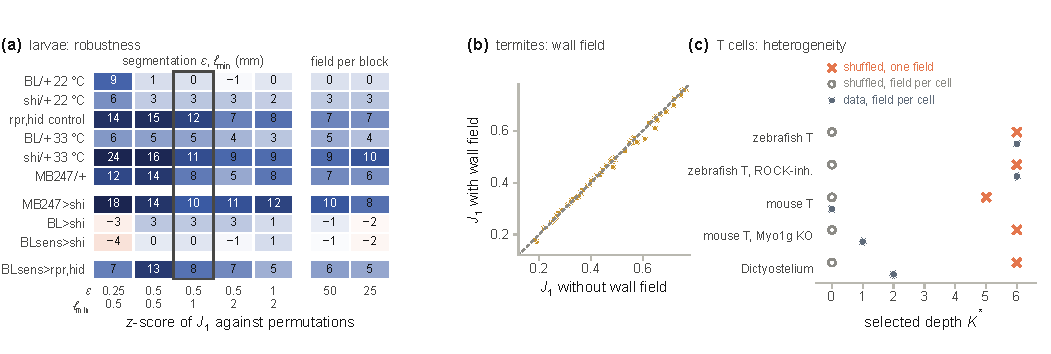
\includegraphics[width=\textwidth]{figs/figA4_controls.pdf}
\caption{Controls on real walkers. (a)~\emph{Drosophila} larvae: $z$-score of $J_1$ against permutation nulls for five segmentation settings (corridor half-width $\varepsilon$ and $\lmin$, in mm; boxed, the setting of Table~\ref{tab:larvae}), and with fields re-estimated every 50 or 25 flights, against permutations within blocks. (b)~Termites: lag-1 coupling of a $K=1$ fit with and without a wall field (band of 6\,mm), one point per termite. (c)~T cells and \emph{Dictyostelium}~\cite{Jerison2020}: depth selected after shuffling the steps within each cell, with a common field (crosses) or one field per cell (open circles), and on the real data with one field per cell (filled).}
\label{fig:controls}
\end{figure*}

\paragraph{Preprocessing.} Table~\ref{tab:datasets} lists the data. For the larvae, flights below $\lmin=1$\,mm (5--13\% of all flights, 28\% for the two lines with silenced or ablated sensory neurons) are set to $\lmin$, and $\lmax$ is the longest flight of the condition. For the termites, $\lmax$ is the longest flight of each track (26--45\,mm), and the wall state of a flight is the fraction of its points within 3, 6 or 9\,mm of the wall, the arena being estimated from the track as the circle that contains 99.5\% of its points. For the T cells the variable is the displacement per frame, with $\lmin$ at the 5th percentile. For the collective analyses, $\lmin$ is at the localization floor (5th percentile) and steps above the 99.95th percentile are treated as tracking glitches. Baboon positions are taken every 10\,s (every 30\,s for the robustness check) and pigeon positions every second, keeping the first fix of each second for the birds logged at 5\,Hz. A heading is defined for steps of at least 1\,m (baboons, about four times the GPS error) or 3\,m (pigeons); a unit that moves less contributes a zero vector to its own lags and to its neighbors' regressors. Each day (baboons) or release (pigeons) is a co-recorded group, with its own unit and time fields.

\paragraph{Larvae.} Table~\ref{tab:larvae} details the ten conditions. The memory does not depend on the segmentation, with $\varepsilon\in\{0.25,0.5,1\}$\,mm and $\lmin\in\{0.5,1,2\}$\,mm, and in six of the seven conditions with memory it survives fields re-estimated every 50 or 25 flights [\figref{fig:controls}(a)]; in BL$>$shi it does not. Over the full range $[\lmin,\lmax]$ a truncated log-normal law, the MaxEnt law with $\langle x^2\rangle$ also fixed, describes the histogram better than a truncated power law in eight conditions out of ten ($\Delta$BIC$\,=286$--1625); the power law is competitive only for the larvae with silenced or ablated sensory neurons. This does not contradict tail fits above a data-chosen $x_{\min}$~\cite{Clauset2009}, but ``L\'evy'' here refers to two decades at most. The memory is the same with either single-flight law (Table~\ref{tab:larvae}, $z_{25}$).

\paragraph{Termites and the wall.} With the wall state of each flight as a covariate, the lag-1 coupling is unchanged in every termite [\figref{fig:controls}(b)]. The wall field improves BIC by a few units for the typical termite (median $-3.5$ at 6\,mm) and by much more for a few, without affecting their memory.

\paragraph{T cells.} With a common field, shuffled T cells select $K^*=5$--6 in 49 of 50 surrogates, the maximal depth in 43; with one field per cell, $K^*=0$ in every surrogate [\figref{fig:controls}(c)]. The steps are log-normal rather than power-law distributed, by $10^2$--$10^4$ BIC units.

% -----------------------------------------------------------------------------
\section{The collective model}\label{app:collective}

\begin{figure*}[t]
\centering
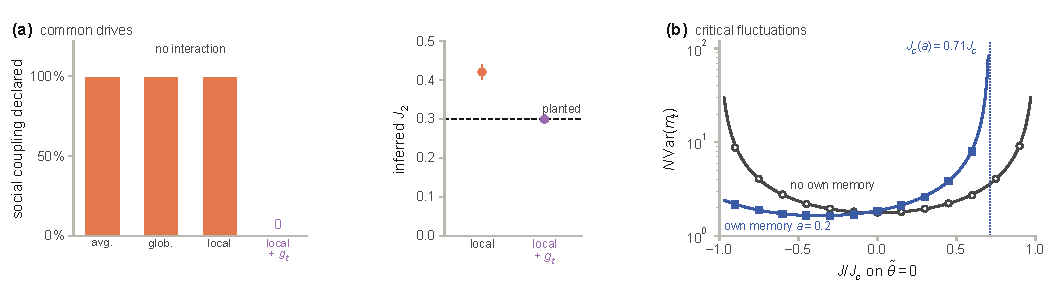
\includegraphics[width=\textwidth]{figs/figA5_collective.pdf}
\caption{Synthetic collectives. (a)~A drive common to all units, without interaction (40 replicates): fraction of data sets in which a social coupling is declared by the group-average analysis, by a global coupling, by a local coupling, and by a local coupling with time fields; right, a planted local coupling $J_2=0.3$ under the same drive, inferred without and with time fields (mean $\pm$ s.d.). (b)~Fluctuations of the collective log-speed versus $J$ on the line $\tilde\theta=0$, without (open circles) and with own memory $a=0.2$ (squares); lines, the theory of Sec.~\ref{sec:meanfield}; dotted, the shifted threshold $J_c(a)=0.71J_c$. $L=\ln100$.}
\label{fig:collective}
\end{figure*}

\begin{table*}[t]
\caption{Synthetic collectives: the analysis of the group average of Ref.~\cite{Agliari2024} (depth $\tau_M^*$ selected by AIC, delay given by $\arg\max_\tau|J_\tau|$) against the self\,+\,social model~\eqref{eq:selfsocial} (depths by BIC). ``Declared'': a nonzero social coupling is selected. Speed-Vicsek model, $L=\ln100$, 1500 frames, $N=50$ unless stated; replicates in parentheses.}
\label{tab:collective}
\begin{ruledtabular}
\begin{tabular}{>{\raggedright\arraybackslash}p{5.0cm}>{\raggedright\arraybackslash}p{5.6cm}>{\raggedright\arraybackslash}p{5.6cm}}
experiment & group average & self\,+\,social\\
\colrule
own memory $a=(0.25,0.10)$, local $J_3=0.35$ (40) & delay 3 in 22/40, 1 in 13/40; spurious $J_1=0.28$, $J_2=0.12$ & $(K_s^*,K_c^*)=(2,3)$ in 38/40; $\hat a=(0.245,0.095)$, $\hat J_3=0.348\pm0.024$\\
own memory of depth 3, no interaction ($N=10$, 30, 100; 40 each) & declared in 100\% (exact likelihood: 97--100\%) & declared in 1/120; $K_s^*=3$ in 116/120\\
common drive, no interaction (40) & declared in 100\% & global 100\%, local 100\%, local with time fields 0\%\\
common drive, local $J_2=0.3$ (40) & declared in 100\% & local: $\hat J_2=0.42$; local with time fields: $\hat J_2=0.300\pm0.012$\\
group-average model true, $J_1=0.25$, $J_4=0.35$ ($N=5$--100; 60 each) & $\hat J_4=0.43\pm0.06$ at $N=5$, $0.35\pm0.04$ at $N=100$ & exact likelihood: $\hat J_4=0.34\pm0.03$ at $N=5$, $0.35\pm0.04$ at $N=100$\\
own memory, local delay $\Delta=1,2,4,6$ (30 each) & delay recovered in 100, 73, 40, 17\% & delay recovered in 100\% for every $\Delta$\\
directions, persistent turning, no interaction (30) & declared in 30/30 (delay 1) & declared in 0/30\\
directions, persistence and local $J_3$ (30) & delay 3 in 0/30 (always 1) & declared in 30/30, delay 3 in 30/30\\
\end{tabular}
\end{ruledtabular}
\end{table*}

\paragraph{Estimation.} The self\,+\,social model~\eqref{eq:selfsocial} is fitted by Newton's method with a sparse Hessian (unit and time fields) and a dense block for the shared couplings. The block of the time fields is diagonal, because each row belongs to one frame, so each Newton step eliminates it exactly (a Schur complement) and solves the remaining dense system for unit fields and couplings, a few hundred parameters; with $6\times10^4$ time fields (baboons at 10\,s) a fit takes seconds, with the same optimum and standard errors as a sparse factorization. Unit and time fields have one flat direction per co-recorded group, $h_i\to h_i+\Delta$, $g_t\to g_t-\Delta$, fixed by a vanishing ridge on the $g_t$; the flat directions are common to all models compared, so BIC differences are unaffected. Self and social depths are selected jointly by BIC on common rows. For directions, $p(\bm n_i^t|\text{past})\propto e^{\bm\theta_i^t\cdot\bm n_i^t}$ is a von Mises law~\cite{MardiaJupp2000} for the unit vector $\bm n_i^t$ of the step, with $\bm\theta_i^t=\mathbf h_i+\mathbf g_t+\sum_\tau a_\tau\bm n_i^{t-\tau}+\sum_\tau J_\tau\bm s_i^{t-\tau}$, the planar spin of Ref.~\cite{Agliari2024}, where $\bm s_i^{t-\tau}$ is the mean unit vector of the neighbors; its negative log-likelihood $\sum[\ln I_0(|\bm\theta|)-\bm\theta\cdot\bm n]$ is convex, and the time-field block is two-by-two block diagonal.

\paragraph{Exactness of the mean-field measure.} The measure $P_A$ of Ref.~\cite{Agliari2024} factorizes over units and frames with one-body weights $e^{x_i^t\theta_t}/Z(\theta_t)$, the first $\tau_M$ frames being fixed by delta functions; evaluated at the data it is $\prod_{t,i}p(x_i^t|\text{past})$ with $\theta_t=H+\sum_\tau J_\tau m^E_{t-\tau}$. Concavity follows as for Eq.~\eqref{eq:loglik}. The stationarity conditions $\sum_{t,i}[x_i^t-\Lambda(\theta_t)]=0$ and $\sum_{t,i}[x_i^t-\Lambda(\theta_t)]m_{t-\tau}=0$ characterize the exact estimator, whereas the original implementation~\cite{Agliari2024} imposes $\Lambda(\theta_t)\simeq m_t$ frame by frame and solves it by least squares after the inversion $G_t=\Lambda^{-1}(m_t)$, a convenient moment approximation.

\paragraph{Aggregation.} Let units be conditionally independent given their own pasts and jointly stationary. For a model of the group average alone, the expected score for $J_\tau$ at $J=0$ is $\E[\sum_i(x_i^t-\bar m)m_{t-\tau}]=N^{-1}\sum_{i,j}\mathrm{Cov}(x_i^t,x_j^{t-\tau})=\bar C(\tau)$ per frame, of order one: $J=0$ is not a solution whenever there is own memory. Linearizing $G_t\simeq\bar\theta+(m_t-\bar m)/\Lambda'(\bar\theta)$, the regression of $G_t$ on lags of $m$ is $1/\Lambda'$ times the autoregression of $m$ on its own lags; since $\mathrm{Cov}(m_t,m_{t-\tau})=N^{-1}\bar C(\tau)$, the factors $N^{-1}$ cancel in the Yule--Walker equations, which gives Eq.~\eqref{eq:aggregation}. For the self\,+\,social model with leave-one-out regressors, the tower property gives $\E[(x_i^t-\E[x_i^t|x_i^{<t}])\,m^{(-i)}_{t-\tau}]=0$, because $m^{(-i)}$ is independent of unit $i$: the social score vanishes at the truth.

\paragraph{Common drives.} A shared stationary field $u_t$ with autocovariance $C_u$ induces $\mathrm{Cov}(x_i^t,x_j^{t-\tau})\simeq\Lambda'^2C_u(\tau)$ between non-interacting units, to linear order. With unit and time fields, the identity $m^{(-i)}_{t-\tau}=\frac{n}{n-1}m_{t-\tau}-\frac1{n-1}x_i^{t-\tau}$ ($n$ units in the frame) shows that the global regressor is a function of the frame, absorbed by $g_t$, plus a multiple of the own lag. For $\tau\le K_s$ a global coupling is not identifiable (exactly so when $n$ is constant); for $\tau>K_s$ it estimates $-(n-1)$ times the omitted own memory at that lag. A local regressor is not in the span of the time fields and own lags unless all neighborhood means coincide. On synthetic data [\figref{fig:collective}(a)], every reading except local coupling with time fields declares a coupling under a common drive alone, and only that reading recovers a planted local coupling without bias.

\paragraph{Mean-field theory.} By the law of large numbers, $m_t\to\Lambda(H+\sum_\tau J_\tau m_{t-\tau})$. Linearizing around a fixed point gives the characteristic equation $1=\Lambda'(\theta^*)\sum_\tau J_\tau z^{-\tau}$. For non-negative couplings, $f(z)=\Lambda'\sum_\tau J_\tau z^{-\tau}$ is decreasing on $z>0$ and $|f(z)|\le f(|z|)$, so a root with $|z|\ge1$ exists if and only if $f(1)=\Lambda'J_{\rm tot}\ge1$; when the delays have no common divisor the critical root is $z=1$ alone (a fold). Since $\Lambda'\le L^2/12$, with equality at $\theta=0$, bistability requires $J_{\rm tot}>12/L^2$, the cusp being at $\tilde\theta=0$, $m=L/2$. For a single delay $d$ the map decouples into $d$ sub-chains $y^{(r)}_n=m_{nd+r}$ obeying $y_{n+1}=\Lambda(H+Jy_n)$; for $J<0$ each undergoes a flip at $\Lambda'|J|=1$, and a lag-1 term $a_1>0$ in the characteristic equation $z^d=\Lambda'J+\Lambda'a_1z^{d-1}$ favors the in-phase mode, of period $2d$. For finite $N$ and one lag, $\delta m_t=\Lambda'J\delta m_{t-1}+\eta_t$ with $\mathrm{Var}\,\eta=\Lambda'/N$ gives $N\,\mathrm{Var}(m)=\Lambda'/[1-(\Lambda'J)^2]$ [\figref{fig:collective}(b)].

\paragraph{Own memory in mean field.} With lag-1 self coupling $a\ge0$, propagation of chaos makes each unit, at a stationary state $m^*$, an independent chain with field $h_{\rm eff}=H+J_{\rm tot}m^*$ and stationary law $\pi(x)\propto e^{h_{\rm eff}x}Z(h_{\rm eff}+ax)$, Eq.~\eqref{eq:stationary}. The self-consistency is $m^*=\Psi(H+J_{\rm tot}m^*)$, with $\Psi(h)=\E_\pi[x]$, and the symmetry line is $H+(J_{\rm tot}+a)L/2=0$. A field perturbation propagates as $\delta m_t=\sum_{s\ge0}R(s)\,\delta h_{t-s}$, with $R(s)=\mathrm{Cov}(x_s,\epsilon_0)$ the response of one unit, $\epsilon_0=x_0-\E[x_0|\text{past}]$ being the innovation; for $a\ge0$, $R(s)\ge0$, the argument above applies to $1=\hat R(z)\sum_\tau J_\tau z^{-\tau}$, and stability is lost at $J_{\rm tot}\chi=1$ with $\chi=\sum_sR(s)=\partial\Psi/\partial h$. To leading order in $1/N$, $N\,\mathrm{Var}(m)=\int\frac{d\omega}{2\pi}S_x(\omega)|1-\hat J(\omega)\hat R(\omega)|^{-2}$, with $S_x$ the spectrum of one unit. We compute $R$, $S_x$ and $\chi$ from the transition matrix of the chain on 400 Gauss--Legendre nodes.

\paragraph{Synthetic collectives.} The speed-Vicsek model places $N$ units in a periodic box; headings follow Vicsek alignment~\cite{Vicsek1995}, and log-speeds are drawn from Eq.~\eqref{eq:selfsocial} with planted own memory, local (three nearest neighbors) or global couplings and, when stated, a common Ornstein--Uhlenbeck drive; steps are then recomputed from the positions, as in an experiment. Individual fields are drawn from $U(-1.3,-0.5)$. Table~\ref{tab:collective} collects the experiments. Directions behave like speeds: for units with persistent turning and no interaction, the group-average analysis of directions declares delayed interactions in every replicate, the self\,+\,social von Mises model in none. With AIC instead of BIC, the self\,+\,social model itself declares spurious couplings in 27\% of interaction-free data sets, the value of Eq.~\eqref{eq:woodroofe} again.

\paragraph{Time-shift null.} In a time-shift surrogate every unit's track is shifted by an independent random circular offset, which keeps its own memory, heterogeneity and marginal law and destroys every synchrony between units, interactions and common drives alike; a permutation of frames destroys own memory as well, and therefore tests memory and synchrony together.

\paragraph{Neighbors in real groups.} The local regressor of unit $i$ at delay $\tau$ is the mean of the variable over the units of distance ranks $r_0+1,\dots,r_1$ from $i$ at the emission frame $t-\tau$: the three nearest for baboons, and the nearest one for pigeons, whose flocks have three to eight birds in a frame, so that a larger neighborhood would be the whole flock and, as shown above, not identifiable with time fields. The decay with distance is measured by single-neighbor regressors of ranks 1, 2, 3, 6 and 12 (baboons) or 1, 2 and 3 (pigeons), fitted jointly with three delays each; the asymmetry, by splitting the six (baboons) or three (pigeons) nearest neighbors into those ahead of and those behind $i$ along the group heading, the direction of the mean step at $t-\tau$. Anchoring the neighborhood at the current position of $i$ instead (the units that at $t-\tau$ were nearest to where $i$ is now) also picks up fields fixed in space, such as trails, which time fields cannot absorb. In the time-shift null the positions are shifted with the steps, so the neighbors of a shifted unit are whoever passed near the same place at another time: the null removes synchrony but keeps fields fixed in space, and its coupling to the nearest neighbor need not vanish.


\bibliography{refs}

\end{document}
